\documentclass[twoside]{book}

% Packages required by doxygen
\usepackage{fixltx2e}
\usepackage{calc}
\usepackage{doxygen}
\usepackage[export]{adjustbox} % also loads graphicx
\usepackage{graphicx}
\usepackage[utf8]{inputenc}
\usepackage{makeidx}
\usepackage{multicol}
\usepackage{multirow}
\PassOptionsToPackage{warn}{textcomp}
\usepackage{textcomp}
\usepackage[nointegrals]{wasysym}
\usepackage[table]{xcolor}

% Font selection
\usepackage[T1]{fontenc}
\usepackage[scaled=.90]{helvet}
\usepackage{courier}
\usepackage{amssymb}
\usepackage{sectsty}
\renewcommand{\familydefault}{\sfdefault}
\allsectionsfont{%
  \fontseries{bc}\selectfont%
  \color{darkgray}%
}
\renewcommand{\DoxyLabelFont}{%
  \fontseries{bc}\selectfont%
  \color{darkgray}%
}
\newcommand{\+}{\discretionary{\mbox{\scriptsize$\hookleftarrow$}}{}{}}

% Page & text layout
\usepackage{geometry}
\geometry{%
  a4paper,%
  top=2.5cm,%
  bottom=2.5cm,%
  left=2.5cm,%
  right=2.5cm%
}
\tolerance=750
\hfuzz=15pt
\hbadness=750
\setlength{\emergencystretch}{15pt}
\setlength{\parindent}{0cm}
\setlength{\parskip}{3ex plus 2ex minus 2ex}
\makeatletter
\renewcommand{\paragraph}{%
  \@startsection{paragraph}{4}{0ex}{-1.0ex}{1.0ex}{%
    \normalfont\normalsize\bfseries\SS@parafont%
  }%
}
\renewcommand{\subparagraph}{%
  \@startsection{subparagraph}{5}{0ex}{-1.0ex}{1.0ex}{%
    \normalfont\normalsize\bfseries\SS@subparafont%
  }%
}
\makeatother

% Headers & footers
\usepackage{fancyhdr}
\pagestyle{fancyplain}
\fancyhead[LE]{\fancyplain{}{\bfseries\thepage}}
\fancyhead[CE]{\fancyplain{}{}}
\fancyhead[RE]{\fancyplain{}{\bfseries\leftmark}}
\fancyhead[LO]{\fancyplain{}{\bfseries\rightmark}}
\fancyhead[CO]{\fancyplain{}{}}
\fancyhead[RO]{\fancyplain{}{\bfseries\thepage}}
\fancyfoot[LE]{\fancyplain{}{}}
\fancyfoot[CE]{\fancyplain{}{}}
\fancyfoot[RE]{\fancyplain{}{\bfseries\scriptsize Generated by Doxygen }}
\fancyfoot[LO]{\fancyplain{}{\bfseries\scriptsize Generated by Doxygen }}
\fancyfoot[CO]{\fancyplain{}{}}
\fancyfoot[RO]{\fancyplain{}{}}
\renewcommand{\footrulewidth}{0.4pt}
\renewcommand{\chaptermark}[1]{%
  \markboth{#1}{}%
}
\renewcommand{\sectionmark}[1]{%
  \markright{\thesection\ #1}%
}

% Indices & bibliography
\usepackage{natbib}
\usepackage[titles]{tocloft}
\setcounter{tocdepth}{3}
\setcounter{secnumdepth}{5}
\makeindex

% Hyperlinks (required, but should be loaded last)
\usepackage{ifpdf}
\ifpdf
  \usepackage[pdftex,pagebackref=true]{hyperref}
\else
  \usepackage[ps2pdf,pagebackref=true]{hyperref}
\fi
\hypersetup{%
  colorlinks=true,%
  linkcolor=blue,%
  citecolor=blue,%
  unicode%
}

% Custom commands
\newcommand{\clearemptydoublepage}{%
  \newpage{\pagestyle{empty}\cleardoublepage}%
}

\usepackage{caption}
\captionsetup{labelsep=space,justification=centering,font={bf},singlelinecheck=off,skip=4pt,position=top}

%===== C O N T E N T S =====

\begin{document}

% Titlepage & ToC
\hypersetup{pageanchor=false,
             bookmarksnumbered=true,
             pdfencoding=unicode
            }
\pagenumbering{alph}
\begin{titlepage}
\vspace*{7cm}
\begin{center}%
{\Large Project 1 \\[1ex]\large 1.\+0 }\\
\vspace*{1cm}
{\large Generated by Doxygen 1.8.14}\\
\end{center}
\end{titlepage}
\clearemptydoublepage
\pagenumbering{roman}
\tableofcontents
\clearemptydoublepage
\pagenumbering{arabic}
\hypersetup{pageanchor=true}

%--- Begin generated contents ---
\chapter{Namespace Index}
\section{Packages}
Here are the packages with brief descriptions (if available)\+:\begin{DoxyCompactList}
\item\contentsline{section}{\mbox{\hyperlink{namespace_b_s_k___encryption}{B\+S\+K\+\_\+\+Encryption}} }{\pageref{namespace_b_s_k___encryption}}{}
\item\contentsline{section}{\mbox{\hyperlink{namespace_b_s_k___encryption_1_1_converters}{B\+S\+K\+\_\+\+Encryption.\+Converters}} }{\pageref{namespace_b_s_k___encryption_1_1_converters}}{}
\item\contentsline{section}{\mbox{\hyperlink{namespace_b_s_k___encryption_1_1_encryption}{B\+S\+K\+\_\+\+Encryption.\+Encryption}} }{\pageref{namespace_b_s_k___encryption_1_1_encryption}}{}
\item\contentsline{section}{\mbox{\hyperlink{namespace_b_s_k___encryption_1_1_encryption_1_1_o_f_b}{B\+S\+K\+\_\+\+Encryption.\+Encryption.\+O\+FB}} }{\pageref{namespace_b_s_k___encryption_1_1_encryption_1_1_o_f_b}}{}
\item\contentsline{section}{\mbox{\hyperlink{namespace_b_s_k___encryption_1_1_properties}{B\+S\+K\+\_\+\+Encryption.\+Properties}} }{\pageref{namespace_b_s_k___encryption_1_1_properties}}{}
\item\contentsline{section}{\mbox{\hyperlink{namespace_b_s_k___encryption_1_1_validators}{B\+S\+K\+\_\+\+Encryption.\+Validators}} }{\pageref{namespace_b_s_k___encryption_1_1_validators}}{}
\item\contentsline{section}{\mbox{\hyperlink{namespace_b_s_k___encryption_1_1_view_models}{B\+S\+K\+\_\+\+Encryption.\+View\+Models}} }{\pageref{namespace_b_s_k___encryption_1_1_view_models}}{}
\item\contentsline{section}{\mbox{\hyperlink{namespace_b_s_k___encryption_1_1_windows}{B\+S\+K\+\_\+\+Encryption.\+Windows}} }{\pageref{namespace_b_s_k___encryption_1_1_windows}}{}
\item\contentsline{section}{\mbox{\hyperlink{namespace_xaml_generated_namespace}{Xaml\+Generated\+Namespace}} }{\pageref{namespace_xaml_generated_namespace}}{}
\end{DoxyCompactList}

\chapter{Hierarchical Index}
\section{Class Hierarchy}
This inheritance list is sorted roughly, but not completely, alphabetically\+:\begin{DoxyCompactList}
\item \contentsline{section}{B\+S\+K\+\_\+\+Encryption.\+Encryption.\+Aes\+Encryption\+Api}{\pageref{class_b_s_k___encryption_1_1_encryption_1_1_aes_encryption_api}}{}
\item Application\begin{DoxyCompactList}
\item \contentsline{section}{B\+S\+K\+\_\+\+Encryption.\+App}{\pageref{class_b_s_k___encryption_1_1_app}}{}
\item \contentsline{section}{B\+S\+K\+\_\+\+Encryption.\+App}{\pageref{class_b_s_k___encryption_1_1_app}}{}
\item \contentsline{section}{B\+S\+K\+\_\+\+Encryption.\+App}{\pageref{class_b_s_k___encryption_1_1_app}}{}
\end{DoxyCompactList}
\item I\+Component\+Connector\begin{DoxyCompactList}
\item \contentsline{section}{B\+S\+K\+\_\+\+Encryption.\+Windows.\+Decrypte\+Window}{\pageref{class_b_s_k___encryption_1_1_windows_1_1_decrypte_window}}{}
\item \contentsline{section}{B\+S\+K\+\_\+\+Encryption.\+Windows.\+Decrypte\+Window}{\pageref{class_b_s_k___encryption_1_1_windows_1_1_decrypte_window}}{}
\item \contentsline{section}{B\+S\+K\+\_\+\+Encryption.\+Windows.\+Encrypte\+Window}{\pageref{class_b_s_k___encryption_1_1_windows_1_1_encrypte_window}}{}
\item \contentsline{section}{B\+S\+K\+\_\+\+Encryption.\+Windows.\+Encrypte\+Window}{\pageref{class_b_s_k___encryption_1_1_windows_1_1_encrypte_window}}{}
\item \contentsline{section}{B\+S\+K\+\_\+\+Encryption.\+Windows.\+Main\+Window}{\pageref{class_b_s_k___encryption_1_1_windows_1_1_main_window}}{}
\item \contentsline{section}{B\+S\+K\+\_\+\+Encryption.\+Windows.\+Main\+Window}{\pageref{class_b_s_k___encryption_1_1_windows_1_1_main_window}}{}
\item \contentsline{section}{B\+S\+K\+\_\+\+Encryption.\+Windows.\+Register\+Window}{\pageref{class_b_s_k___encryption_1_1_windows_1_1_register_window}}{}
\item \contentsline{section}{B\+S\+K\+\_\+\+Encryption.\+Windows.\+Register\+Window}{\pageref{class_b_s_k___encryption_1_1_windows_1_1_register_window}}{}
\item \contentsline{section}{B\+S\+K\+\_\+\+Encryption.\+Windows.\+Users\+Window}{\pageref{class_b_s_k___encryption_1_1_windows_1_1_users_window}}{}
\item \contentsline{section}{B\+S\+K\+\_\+\+Encryption.\+Windows.\+Users\+Window}{\pageref{class_b_s_k___encryption_1_1_windows_1_1_users_window}}{}
\end{DoxyCompactList}
\item I\+Notify\+Property\+Changed\begin{DoxyCompactList}
\item \contentsline{section}{B\+S\+K\+\_\+\+Encryption.\+View\+Models.\+Notify\+Property\+Changed}{\pageref{class_b_s_k___encryption_1_1_view_models_1_1_notify_property_changed}}{}
\begin{DoxyCompactList}
\item \contentsline{section}{B\+S\+K\+\_\+\+Encryption.\+View\+Models.\+Data\+View\+Model}{\pageref{class_b_s_k___encryption_1_1_view_models_1_1_data_view_model}}{}
\begin{DoxyCompactList}
\item \contentsline{section}{B\+S\+K\+\_\+\+Encryption.\+View\+Models.\+Decrypte\+Data\+View\+Model}{\pageref{class_b_s_k___encryption_1_1_view_models_1_1_decrypte_data_view_model}}{}
\item \contentsline{section}{B\+S\+K\+\_\+\+Encryption.\+View\+Models.\+Encrypte\+Data\+View\+Model}{\pageref{class_b_s_k___encryption_1_1_view_models_1_1_encrypte_data_view_model}}{}
\end{DoxyCompactList}
\end{DoxyCompactList}
\end{DoxyCompactList}
\item Internal\+Type\+Helper\begin{DoxyCompactList}
\item \contentsline{section}{Xaml\+Generated\+Namespace.\+Generated\+Internal\+Type\+Helper}{\pageref{class_xaml_generated_namespace_1_1_generated_internal_type_helper}}{}
\item \contentsline{section}{Xaml\+Generated\+Namespace.\+Generated\+Internal\+Type\+Helper}{\pageref{class_xaml_generated_namespace_1_1_generated_internal_type_helper}}{}
\end{DoxyCompactList}
\item I\+Value\+Converter\begin{DoxyCompactList}
\item \contentsline{section}{B\+S\+K\+\_\+\+Encryption.\+Converters.\+Block\+Converter}{\pageref{class_b_s_k___encryption_1_1_converters_1_1_block_converter}}{}
\item \contentsline{section}{B\+S\+K\+\_\+\+Encryption.\+Converters.\+Cipher\+Converter}{\pageref{class_b_s_k___encryption_1_1_converters_1_1_cipher_converter}}{}
\end{DoxyCompactList}
\item \contentsline{section}{B\+S\+K\+\_\+\+Encryption.\+Encryption.\+Rsa\+Encryption\+Api}{\pageref{class_b_s_k___encryption_1_1_encryption_1_1_rsa_encryption_api}}{}
\item \contentsline{section}{B\+S\+K\+\_\+\+Encryption.\+Encryption.\+S\+H\+A256\+Encryption\+Api}{\pageref{class_b_s_k___encryption_1_1_encryption_1_1_s_h_a256_encryption_api}}{}
\item Stream\begin{DoxyCompactList}
\item \contentsline{section}{B\+S\+K\+\_\+\+Encryption.\+Encryption.\+O\+F\+B.\+O\+F\+B\+Stream}{\pageref{class_b_s_k___encryption_1_1_encryption_1_1_o_f_b_1_1_o_f_b_stream}}{}
\item \contentsline{section}{B\+S\+K\+\_\+\+Encryption.\+Encryption.\+O\+F\+B.\+Zero\+Stream}{\pageref{class_b_s_k___encryption_1_1_encryption_1_1_o_f_b_1_1_zero_stream}}{}
\end{DoxyCompactList}
\item \contentsline{section}{B\+S\+K\+\_\+\+Encryption.\+Encryption.\+User}{\pageref{class_b_s_k___encryption_1_1_encryption_1_1_user}}{}
\item \contentsline{section}{B\+S\+K\+\_\+\+Encryption.\+View\+Models.\+User\+Grid\+Element}{\pageref{class_b_s_k___encryption_1_1_view_models_1_1_user_grid_element}}{}
\item \contentsline{section}{B\+S\+K\+\_\+\+Encryption.\+View\+Models.\+User\+View\+Model}{\pageref{class_b_s_k___encryption_1_1_view_models_1_1_user_view_model}}{}
\item Validation\+Rule\begin{DoxyCompactList}
\item \contentsline{section}{B\+S\+K\+\_\+\+Encryption.\+Validators.\+Input\+Path\+Validator}{\pageref{class_b_s_k___encryption_1_1_validators_1_1_input_path_validator}}{}
\item \contentsline{section}{B\+S\+K\+\_\+\+Encryption.\+Validators.\+Output\+Path\+Validator}{\pageref{class_b_s_k___encryption_1_1_validators_1_1_output_path_validator}}{}
\item \contentsline{section}{B\+S\+K\+\_\+\+Encryption.\+Validators.\+Text\+Validator}{\pageref{class_b_s_k___encryption_1_1_validators_1_1_text_validator}}{}
\end{DoxyCompactList}
\item Window\begin{DoxyCompactList}
\item \contentsline{section}{B\+S\+K\+\_\+\+Encryption.\+Windows.\+Decrypte\+Window}{\pageref{class_b_s_k___encryption_1_1_windows_1_1_decrypte_window}}{}
\item \contentsline{section}{B\+S\+K\+\_\+\+Encryption.\+Windows.\+Decrypte\+Window}{\pageref{class_b_s_k___encryption_1_1_windows_1_1_decrypte_window}}{}
\item \contentsline{section}{B\+S\+K\+\_\+\+Encryption.\+Windows.\+Decrypte\+Window}{\pageref{class_b_s_k___encryption_1_1_windows_1_1_decrypte_window}}{}
\item \contentsline{section}{B\+S\+K\+\_\+\+Encryption.\+Windows.\+Encrypte\+Window}{\pageref{class_b_s_k___encryption_1_1_windows_1_1_encrypte_window}}{}
\item \contentsline{section}{B\+S\+K\+\_\+\+Encryption.\+Windows.\+Encrypte\+Window}{\pageref{class_b_s_k___encryption_1_1_windows_1_1_encrypte_window}}{}
\item \contentsline{section}{B\+S\+K\+\_\+\+Encryption.\+Windows.\+Encrypte\+Window}{\pageref{class_b_s_k___encryption_1_1_windows_1_1_encrypte_window}}{}
\item \contentsline{section}{B\+S\+K\+\_\+\+Encryption.\+Windows.\+Main\+Window}{\pageref{class_b_s_k___encryption_1_1_windows_1_1_main_window}}{}
\item \contentsline{section}{B\+S\+K\+\_\+\+Encryption.\+Windows.\+Main\+Window}{\pageref{class_b_s_k___encryption_1_1_windows_1_1_main_window}}{}
\item \contentsline{section}{B\+S\+K\+\_\+\+Encryption.\+Windows.\+Main\+Window}{\pageref{class_b_s_k___encryption_1_1_windows_1_1_main_window}}{}
\item \contentsline{section}{B\+S\+K\+\_\+\+Encryption.\+Windows.\+Register\+Window}{\pageref{class_b_s_k___encryption_1_1_windows_1_1_register_window}}{}
\item \contentsline{section}{B\+S\+K\+\_\+\+Encryption.\+Windows.\+Register\+Window}{\pageref{class_b_s_k___encryption_1_1_windows_1_1_register_window}}{}
\item \contentsline{section}{B\+S\+K\+\_\+\+Encryption.\+Windows.\+Register\+Window}{\pageref{class_b_s_k___encryption_1_1_windows_1_1_register_window}}{}
\item \contentsline{section}{B\+S\+K\+\_\+\+Encryption.\+Windows.\+Users\+Window}{\pageref{class_b_s_k___encryption_1_1_windows_1_1_users_window}}{}
\item \contentsline{section}{B\+S\+K\+\_\+\+Encryption.\+Windows.\+Users\+Window}{\pageref{class_b_s_k___encryption_1_1_windows_1_1_users_window}}{}
\end{DoxyCompactList}
\item Window\begin{DoxyCompactList}
\item \contentsline{section}{B\+S\+K\+\_\+\+Encryption.\+Windows.\+Users\+Window}{\pageref{class_b_s_k___encryption_1_1_windows_1_1_users_window}}{}
\end{DoxyCompactList}
\end{DoxyCompactList}

\chapter{Class Index}
\section{Class List}
Here are the classes, structs, unions and interfaces with brief descriptions\+:\begin{DoxyCompactList}
\item\contentsline{section}{\mbox{\hyperlink{class_b_s_k___encryption_1_1_encryption_1_1_aes_encryption_api}{B\+S\+K\+\_\+\+Encryption.\+Encryption.\+Aes\+Encryption\+Api}} \\*Api that gives C\+BC, E\+CB, C\+FB, \mbox{\hyperlink{namespace_b_s_k___encryption_1_1_encryption_1_1_o_f_b}{O\+FB}} Crypto options by merging diffrent implementation form internet. }{\pageref{class_b_s_k___encryption_1_1_encryption_1_1_aes_encryption_api}}{}
\item\contentsline{section}{\mbox{\hyperlink{class_b_s_k___encryption_1_1_app}{B\+S\+K\+\_\+\+Encryption.\+App}} \\*Interaction logic for App.\+xaml }{\pageref{class_b_s_k___encryption_1_1_app}}{}
\item\contentsline{section}{\mbox{\hyperlink{class_b_s_k___encryption_1_1_converters_1_1_block_converter}{B\+S\+K\+\_\+\+Encryption.\+Converters.\+Block\+Converter}} \\*Converts int to string and back. }{\pageref{class_b_s_k___encryption_1_1_converters_1_1_block_converter}}{}
\item\contentsline{section}{\mbox{\hyperlink{class_b_s_k___encryption_1_1_converters_1_1_cipher_converter}{B\+S\+K\+\_\+\+Encryption.\+Converters.\+Cipher\+Converter}} \\*Converts to int from Cipher\+Mode and back. }{\pageref{class_b_s_k___encryption_1_1_converters_1_1_cipher_converter}}{}
\item\contentsline{section}{\mbox{\hyperlink{class_b_s_k___encryption_1_1_view_models_1_1_data_view_model}{B\+S\+K\+\_\+\+Encryption.\+View\+Models.\+Data\+View\+Model}} \\*Context for Cryptography. }{\pageref{class_b_s_k___encryption_1_1_view_models_1_1_data_view_model}}{}
\item\contentsline{section}{\mbox{\hyperlink{class_b_s_k___encryption_1_1_view_models_1_1_decrypte_data_view_model}{B\+S\+K\+\_\+\+Encryption.\+View\+Models.\+Decrypte\+Data\+View\+Model}} \\*Decrypt context model. }{\pageref{class_b_s_k___encryption_1_1_view_models_1_1_decrypte_data_view_model}}{}
\item\contentsline{section}{\mbox{\hyperlink{class_b_s_k___encryption_1_1_windows_1_1_decrypte_window}{B\+S\+K\+\_\+\+Encryption.\+Windows.\+Decrypte\+Window}} \\*\mbox{\hyperlink{class_b_s_k___encryption_1_1_windows_1_1_decrypte_window}{Decrypte\+Window}} }{\pageref{class_b_s_k___encryption_1_1_windows_1_1_decrypte_window}}{}
\item\contentsline{section}{\mbox{\hyperlink{class_b_s_k___encryption_1_1_view_models_1_1_encrypte_data_view_model}{B\+S\+K\+\_\+\+Encryption.\+View\+Models.\+Encrypte\+Data\+View\+Model}} \\*Encrypt context model. }{\pageref{class_b_s_k___encryption_1_1_view_models_1_1_encrypte_data_view_model}}{}
\item\contentsline{section}{\mbox{\hyperlink{class_b_s_k___encryption_1_1_windows_1_1_encrypte_window}{B\+S\+K\+\_\+\+Encryption.\+Windows.\+Encrypte\+Window}} \\*\mbox{\hyperlink{class_b_s_k___encryption_1_1_windows_1_1_encrypte_window}{Encrypte\+Window}} }{\pageref{class_b_s_k___encryption_1_1_windows_1_1_encrypte_window}}{}
\item\contentsline{section}{\mbox{\hyperlink{class_xaml_generated_namespace_1_1_generated_internal_type_helper}{Xaml\+Generated\+Namespace.\+Generated\+Internal\+Type\+Helper}} \\*\mbox{\hyperlink{class_xaml_generated_namespace_1_1_generated_internal_type_helper}{Generated\+Internal\+Type\+Helper}} }{\pageref{class_xaml_generated_namespace_1_1_generated_internal_type_helper}}{}
\item\contentsline{section}{\mbox{\hyperlink{class_b_s_k___encryption_1_1_validators_1_1_input_path_validator}{B\+S\+K\+\_\+\+Encryption.\+Validators.\+Input\+Path\+Validator}} \\*Validator for path }{\pageref{class_b_s_k___encryption_1_1_validators_1_1_input_path_validator}}{}
\item\contentsline{section}{\mbox{\hyperlink{class_b_s_k___encryption_1_1_windows_1_1_main_window}{B\+S\+K\+\_\+\+Encryption.\+Windows.\+Main\+Window}} \\*\mbox{\hyperlink{class_b_s_k___encryption_1_1_windows_1_1_main_window}{Main\+Window}} }{\pageref{class_b_s_k___encryption_1_1_windows_1_1_main_window}}{}
\item\contentsline{section}{\mbox{\hyperlink{class_b_s_k___encryption_1_1_view_models_1_1_notify_property_changed}{B\+S\+K\+\_\+\+Encryption.\+View\+Models.\+Notify\+Property\+Changed}} }{\pageref{class_b_s_k___encryption_1_1_view_models_1_1_notify_property_changed}}{}
\item\contentsline{section}{\mbox{\hyperlink{class_b_s_k___encryption_1_1_encryption_1_1_o_f_b_1_1_o_f_b_stream}{B\+S\+K\+\_\+\+Encryption.\+Encryption.\+O\+F\+B.\+O\+F\+B\+Stream}} \\*Extension to the Rijandael\+Managed for using \mbox{\hyperlink{namespace_b_s_k___encryption_1_1_encryption_1_1_o_f_b}{O\+FB}} mode. }{\pageref{class_b_s_k___encryption_1_1_encryption_1_1_o_f_b_1_1_o_f_b_stream}}{}
\item\contentsline{section}{\mbox{\hyperlink{class_b_s_k___encryption_1_1_validators_1_1_output_path_validator}{B\+S\+K\+\_\+\+Encryption.\+Validators.\+Output\+Path\+Validator}} \\*Validation for output path. }{\pageref{class_b_s_k___encryption_1_1_validators_1_1_output_path_validator}}{}
\item\contentsline{section}{\mbox{\hyperlink{class_b_s_k___encryption_1_1_windows_1_1_register_window}{B\+S\+K\+\_\+\+Encryption.\+Windows.\+Register\+Window}} \\*\mbox{\hyperlink{class_b_s_k___encryption_1_1_windows_1_1_register_window}{Register\+Window}} }{\pageref{class_b_s_k___encryption_1_1_windows_1_1_register_window}}{}
\item\contentsline{section}{\mbox{\hyperlink{class_b_s_k___encryption_1_1_encryption_1_1_rsa_encryption_api}{B\+S\+K\+\_\+\+Encryption.\+Encryption.\+Rsa\+Encryption\+Api}} \\*Api that handles Rsa \mbox{\hyperlink{namespace_b_s_k___encryption_1_1_encryption}{Encryption}} using keys for given user. \mbox{\hyperlink{namespace_b_s_k___encryption_1_1_encryption}{Encryption}} many to one. }{\pageref{class_b_s_k___encryption_1_1_encryption_1_1_rsa_encryption_api}}{}
\item\contentsline{section}{\mbox{\hyperlink{class_b_s_k___encryption_1_1_encryption_1_1_s_h_a256_encryption_api}{B\+S\+K\+\_\+\+Encryption.\+Encryption.\+S\+H\+A256\+Encryption\+Api}} \\*Api that handles the hasing method. }{\pageref{class_b_s_k___encryption_1_1_encryption_1_1_s_h_a256_encryption_api}}{}
\item\contentsline{section}{\mbox{\hyperlink{class_b_s_k___encryption_1_1_validators_1_1_text_validator}{B\+S\+K\+\_\+\+Encryption.\+Validators.\+Text\+Validator}} \\*Validation for path if aren\textquotesingle{}t empty or null. }{\pageref{class_b_s_k___encryption_1_1_validators_1_1_text_validator}}{}
\item\contentsline{section}{\mbox{\hyperlink{class_b_s_k___encryption_1_1_encryption_1_1_user}{B\+S\+K\+\_\+\+Encryption.\+Encryption.\+User}} \\*Container for user/\+Rsa\+\_\+password manage. }{\pageref{class_b_s_k___encryption_1_1_encryption_1_1_user}}{}
\item\contentsline{section}{\mbox{\hyperlink{class_b_s_k___encryption_1_1_view_models_1_1_user_grid_element}{B\+S\+K\+\_\+\+Encryption.\+View\+Models.\+User\+Grid\+Element}} \\*Part of Users selection table. }{\pageref{class_b_s_k___encryption_1_1_view_models_1_1_user_grid_element}}{}
\item\contentsline{section}{\mbox{\hyperlink{class_b_s_k___encryption_1_1_windows_1_1_users_window}{B\+S\+K\+\_\+\+Encryption.\+Windows.\+Users\+Window}} \\*\mbox{\hyperlink{class_b_s_k___encryption_1_1_windows_1_1_users_window}{Users\+Window}} }{\pageref{class_b_s_k___encryption_1_1_windows_1_1_users_window}}{}
\item\contentsline{section}{\mbox{\hyperlink{class_b_s_k___encryption_1_1_view_models_1_1_user_view_model}{B\+S\+K\+\_\+\+Encryption.\+View\+Models.\+User\+View\+Model}} \\*Singleton to remember authorized users in process. }{\pageref{class_b_s_k___encryption_1_1_view_models_1_1_user_view_model}}{}
\item\contentsline{section}{\mbox{\hyperlink{class_b_s_k___encryption_1_1_encryption_1_1_o_f_b_1_1_zero_stream}{B\+S\+K\+\_\+\+Encryption.\+Encryption.\+O\+F\+B.\+Zero\+Stream}} \\*Infinite Stream tha gives always zeros. }{\pageref{class_b_s_k___encryption_1_1_encryption_1_1_o_f_b_1_1_zero_stream}}{}
\end{DoxyCompactList}

\chapter{Namespace Documentation}
\hypertarget{namespace_b_s_k___encryption}{}\section{B\+S\+K\+\_\+\+Encryption Namespace Reference}
\label{namespace_b_s_k___encryption}\index{B\+S\+K\+\_\+\+Encryption@{B\+S\+K\+\_\+\+Encryption}}
\subsection*{Namespaces}
\begin{DoxyCompactItemize}
\end{DoxyCompactItemize}
\subsection*{Classes}
\begin{DoxyCompactItemize}
\item 
class \mbox{\hyperlink{class_b_s_k___encryption_1_1_app}{App}}
\begin{DoxyCompactList}\small\item\em Interaction logic for App.\+xaml \end{DoxyCompactList}\item 
class {\bfseries Const}
\begin{DoxyCompactList}\small\item\em Container for all const that Should be uknown for user. Visible only for the project submit. \end{DoxyCompactList}\end{DoxyCompactItemize}

\hypertarget{namespace_b_s_k___encryption_1_1_converters}{}\section{B\+S\+K\+\_\+\+Encryption.\+Converters Namespace Reference}
\label{namespace_b_s_k___encryption_1_1_converters}\index{B\+S\+K\+\_\+\+Encryption.\+Converters@{B\+S\+K\+\_\+\+Encryption.\+Converters}}
\subsection*{Classes}
\begin{DoxyCompactItemize}
\item 
class \mbox{\hyperlink{class_b_s_k___encryption_1_1_converters_1_1_block_converter}{Block\+Converter}}
\begin{DoxyCompactList}\small\item\em Converts int to string and back. \end{DoxyCompactList}\item 
class \mbox{\hyperlink{class_b_s_k___encryption_1_1_converters_1_1_cipher_converter}{Cipher\+Converter}}
\begin{DoxyCompactList}\small\item\em Converts to int from Cipher\+Mode and back. \end{DoxyCompactList}\end{DoxyCompactItemize}

\hypertarget{namespace_b_s_k___encryption_1_1_encryption}{}\section{B\+S\+K\+\_\+\+Encryption.\+Encryption Namespace Reference}
\label{namespace_b_s_k___encryption_1_1_encryption}\index{B\+S\+K\+\_\+\+Encryption.\+Encryption@{B\+S\+K\+\_\+\+Encryption.\+Encryption}}
\subsection*{Namespaces}
\begin{DoxyCompactItemize}
\end{DoxyCompactItemize}
\subsection*{Classes}
\begin{DoxyCompactItemize}
\item 
class \mbox{\hyperlink{class_b_s_k___encryption_1_1_encryption_1_1_aes_encryption_api}{Aes\+Encryption\+Api}}
\begin{DoxyCompactList}\small\item\em Api that gives C\+BC, E\+CB, C\+FB, \mbox{\hyperlink{namespace_b_s_k___encryption_1_1_encryption_1_1_o_f_b}{O\+FB}} Crypto options by merging diffrent implementation form internet. \end{DoxyCompactList}\item 
class {\bfseries Conversion}
\begin{DoxyCompactList}\small\item\em Handles the conversion form file(string) to functional object. \end{DoxyCompactList}\item 
class \mbox{\hyperlink{class_b_s_k___encryption_1_1_encryption_1_1_rsa_encryption_api}{Rsa\+Encryption\+Api}}
\begin{DoxyCompactList}\small\item\em Api that handles Rsa \mbox{\hyperlink{namespace_b_s_k___encryption_1_1_encryption}{Encryption}} using keys for given user. \mbox{\hyperlink{namespace_b_s_k___encryption_1_1_encryption}{Encryption}} many to one. \end{DoxyCompactList}\item 
class \mbox{\hyperlink{class_b_s_k___encryption_1_1_encryption_1_1_s_h_a256_encryption_api}{S\+H\+A256\+Encryption\+Api}}
\begin{DoxyCompactList}\small\item\em Api that handles the hasing method. \end{DoxyCompactList}\item 
class \mbox{\hyperlink{class_b_s_k___encryption_1_1_encryption_1_1_user}{User}}
\begin{DoxyCompactList}\small\item\em Container for user/\+Rsa\+\_\+password manage. \end{DoxyCompactList}\end{DoxyCompactItemize}

\hypertarget{namespace_b_s_k___encryption_1_1_encryption_1_1_o_f_b}{}\section{B\+S\+K\+\_\+\+Encryption.\+Encryption.\+O\+FB Namespace Reference}
\label{namespace_b_s_k___encryption_1_1_encryption_1_1_o_f_b}\index{B\+S\+K\+\_\+\+Encryption.\+Encryption.\+O\+FB@{B\+S\+K\+\_\+\+Encryption.\+Encryption.\+O\+FB}}
\subsection*{Classes}
\begin{DoxyCompactItemize}
\item 
class \mbox{\hyperlink{class_b_s_k___encryption_1_1_encryption_1_1_o_f_b_1_1_o_f_b_stream}{O\+F\+B\+Stream}}
\begin{DoxyCompactList}\small\item\em Extension to the Rijandael\+Managed for using \mbox{\hyperlink{namespace_b_s_k___encryption_1_1_encryption_1_1_o_f_b}{O\+FB}} mode. \end{DoxyCompactList}\item 
class \mbox{\hyperlink{class_b_s_k___encryption_1_1_encryption_1_1_o_f_b_1_1_zero_stream}{Zero\+Stream}}
\begin{DoxyCompactList}\small\item\em Infinite Stream tha gives always zeros. \end{DoxyCompactList}\end{DoxyCompactItemize}

\hypertarget{namespace_b_s_k___encryption_1_1_properties}{}\section{B\+S\+K\+\_\+\+Encryption.\+Properties Namespace Reference}
\label{namespace_b_s_k___encryption_1_1_properties}\index{B\+S\+K\+\_\+\+Encryption.\+Properties@{B\+S\+K\+\_\+\+Encryption.\+Properties}}
\subsection*{Classes}
\begin{DoxyCompactItemize}
\item 
class {\bfseries Resources}
\begin{DoxyCompactList}\small\item\em A strongly-\/typed resource class, for looking up localized strings, etc. \end{DoxyCompactList}\item 
class {\bfseries Settings}
\end{DoxyCompactItemize}

\hypertarget{namespace_b_s_k___encryption_1_1_validators}{}\section{B\+S\+K\+\_\+\+Encryption.\+Validators Namespace Reference}
\label{namespace_b_s_k___encryption_1_1_validators}\index{B\+S\+K\+\_\+\+Encryption.\+Validators@{B\+S\+K\+\_\+\+Encryption.\+Validators}}
\subsection*{Classes}
\begin{DoxyCompactItemize}
\item 
class \mbox{\hyperlink{class_b_s_k___encryption_1_1_validators_1_1_input_path_validator}{Input\+Path\+Validator}}
\begin{DoxyCompactList}\small\item\em Validator for path \end{DoxyCompactList}\item 
class \mbox{\hyperlink{class_b_s_k___encryption_1_1_validators_1_1_output_path_validator}{Output\+Path\+Validator}}
\begin{DoxyCompactList}\small\item\em Validation for output path. \end{DoxyCompactList}\item 
class \mbox{\hyperlink{class_b_s_k___encryption_1_1_validators_1_1_text_validator}{Text\+Validator}}
\begin{DoxyCompactList}\small\item\em Validation for path if aren\textquotesingle{}t empty or null. \end{DoxyCompactList}\end{DoxyCompactItemize}

\hypertarget{namespace_b_s_k___encryption_1_1_view_models}{}\section{B\+S\+K\+\_\+\+Encryption.\+View\+Models Namespace Reference}
\label{namespace_b_s_k___encryption_1_1_view_models}\index{B\+S\+K\+\_\+\+Encryption.\+View\+Models@{B\+S\+K\+\_\+\+Encryption.\+View\+Models}}
\subsection*{Classes}
\begin{DoxyCompactItemize}
\item 
class \mbox{\hyperlink{class_b_s_k___encryption_1_1_view_models_1_1_data_view_model}{Data\+View\+Model}}
\begin{DoxyCompactList}\small\item\em Context for Cryptography. \end{DoxyCompactList}\item 
class \mbox{\hyperlink{class_b_s_k___encryption_1_1_view_models_1_1_decrypte_data_view_model}{Decrypte\+Data\+View\+Model}}
\begin{DoxyCompactList}\small\item\em Decrypt context model. \end{DoxyCompactList}\item 
class \mbox{\hyperlink{class_b_s_k___encryption_1_1_view_models_1_1_encrypte_data_view_model}{Encrypte\+Data\+View\+Model}}
\begin{DoxyCompactList}\small\item\em Encrypt context model. \end{DoxyCompactList}\item 
class \mbox{\hyperlink{class_b_s_k___encryption_1_1_view_models_1_1_notify_property_changed}{Notify\+Property\+Changed}}
\item 
class \mbox{\hyperlink{class_b_s_k___encryption_1_1_view_models_1_1_user_grid_element}{User\+Grid\+Element}}
\begin{DoxyCompactList}\small\item\em Part of Users selection table. \end{DoxyCompactList}\item 
class \mbox{\hyperlink{class_b_s_k___encryption_1_1_view_models_1_1_user_view_model}{User\+View\+Model}}
\begin{DoxyCompactList}\small\item\em Singleton to remember authorized users in process. \end{DoxyCompactList}\end{DoxyCompactItemize}

\hypertarget{namespace_b_s_k___encryption_1_1_windows}{}\section{B\+S\+K\+\_\+\+Encryption.\+Windows Namespace Reference}
\label{namespace_b_s_k___encryption_1_1_windows}\index{B\+S\+K\+\_\+\+Encryption.\+Windows@{B\+S\+K\+\_\+\+Encryption.\+Windows}}
\subsection*{Classes}
\begin{DoxyCompactItemize}
\item 
class \mbox{\hyperlink{class_b_s_k___encryption_1_1_windows_1_1_decrypte_window}{Decrypte\+Window}}
\begin{DoxyCompactList}\small\item\em \mbox{\hyperlink{class_b_s_k___encryption_1_1_windows_1_1_decrypte_window}{Decrypte\+Window}} \end{DoxyCompactList}\item 
class \mbox{\hyperlink{class_b_s_k___encryption_1_1_windows_1_1_encrypte_window}{Encrypte\+Window}}
\begin{DoxyCompactList}\small\item\em \mbox{\hyperlink{class_b_s_k___encryption_1_1_windows_1_1_encrypte_window}{Encrypte\+Window}} \end{DoxyCompactList}\item 
class \mbox{\hyperlink{class_b_s_k___encryption_1_1_windows_1_1_main_window}{Main\+Window}}
\begin{DoxyCompactList}\small\item\em \mbox{\hyperlink{class_b_s_k___encryption_1_1_windows_1_1_main_window}{Main\+Window}} \end{DoxyCompactList}\item 
class \mbox{\hyperlink{class_b_s_k___encryption_1_1_windows_1_1_register_window}{Register\+Window}}
\begin{DoxyCompactList}\small\item\em \mbox{\hyperlink{class_b_s_k___encryption_1_1_windows_1_1_register_window}{Register\+Window}} \end{DoxyCompactList}\item 
class \mbox{\hyperlink{class_b_s_k___encryption_1_1_windows_1_1_users_window}{Users\+Window}}
\begin{DoxyCompactList}\small\item\em \mbox{\hyperlink{class_b_s_k___encryption_1_1_windows_1_1_users_window}{Users\+Window}} \end{DoxyCompactList}\end{DoxyCompactItemize}

\hypertarget{namespace_xaml_generated_namespace}{}\section{Xaml\+Generated\+Namespace Namespace Reference}
\label{namespace_xaml_generated_namespace}\index{Xaml\+Generated\+Namespace@{Xaml\+Generated\+Namespace}}
\subsection*{Classes}
\begin{DoxyCompactItemize}
\item 
class \mbox{\hyperlink{class_xaml_generated_namespace_1_1_generated_internal_type_helper}{Generated\+Internal\+Type\+Helper}}
\begin{DoxyCompactList}\small\item\em \mbox{\hyperlink{class_xaml_generated_namespace_1_1_generated_internal_type_helper}{Generated\+Internal\+Type\+Helper}} \end{DoxyCompactList}\end{DoxyCompactItemize}

\chapter{Class Documentation}
\hypertarget{class_b_s_k___encryption_1_1_encryption_1_1_aes_encryption_api}{}\section{B\+S\+K\+\_\+\+Encryption.\+Encryption.\+Aes\+Encryption\+Api Class Reference}
\label{class_b_s_k___encryption_1_1_encryption_1_1_aes_encryption_api}\index{B\+S\+K\+\_\+\+Encryption.\+Encryption.\+Aes\+Encryption\+Api@{B\+S\+K\+\_\+\+Encryption.\+Encryption.\+Aes\+Encryption\+Api}}


Api that gives C\+BC, E\+CB, C\+FB, \mbox{\hyperlink{namespace_b_s_k___encryption_1_1_encryption_1_1_o_f_b}{O\+FB}} Crypto options by merging diffrent implementation form internet.  


\subsection*{Public Member Functions}
\begin{DoxyCompactItemize}
\item 
\mbox{\hyperlink{class_b_s_k___encryption_1_1_encryption_1_1_aes_encryption_api_aaeca30b167bea6e2771614e810734002}{Aes\+Encryption\+Api}} (Cipher\+Mode ciphermode, int block\+Size, int key\+Size)
\begin{DoxyCompactList}\small\item\em Constructor that require further initialize method. \end{DoxyCompactList}\item 
\mbox{\hyperlink{class_b_s_k___encryption_1_1_encryption_1_1_aes_encryption_api_a4529e2907b5939d06c0deae23574c909}{Aes\+Encryption\+Api}} (Cipher\+Mode ciphermode, int block\+Size, int key\+Size, byte\mbox{[}$\,$\mbox{]} password)
\begin{DoxyCompactList}\small\item\em Constructor that assign password. \end{DoxyCompactList}\item 
void \mbox{\hyperlink{class_b_s_k___encryption_1_1_encryption_1_1_aes_encryption_api_a89804f5db642dc4abe751635f1af8df7}{Initialize}} ()
\begin{DoxyCompactList}\small\item\em Generates key and IV. \end{DoxyCompactList}\item 
bool \mbox{\hyperlink{class_b_s_k___encryption_1_1_encryption_1_1_aes_encryption_api_a0a40964a924defba499ee3f8c573c87d}{add\+User}} (string name)
\begin{DoxyCompactList}\small\item\em Add user to the approved users. \end{DoxyCompactList}\item 
void \mbox{\hyperlink{class_b_s_k___encryption_1_1_encryption_1_1_aes_encryption_api_a8849055915f670369e4c835bc4b71414}{Write\+To\+Xml}} (Xml\+Writer output)
\begin{DoxyCompactList}\small\item\em Write current object to file using xml standard. \end{DoxyCompactList}\item 
Stream \mbox{\hyperlink{class_b_s_k___encryption_1_1_encryption_1_1_aes_encryption_api_a7a5c47487ff178032ca8c9e4792d0fd5}{Encrypte\+Stream}} (Stream stream)
\begin{DoxyCompactList}\small\item\em Encrypte input stream. \end{DoxyCompactList}\item 
Stream \mbox{\hyperlink{class_b_s_k___encryption_1_1_encryption_1_1_aes_encryption_api_ac15e90b0d83aeaba75361b90d81b7f8b}{Encrypte\+Stream}} (Stream stream, Crypto\+Stream\+Mode mode=Crypto\+Stream\+Mode.\+Read)
\begin{DoxyCompactList}\small\item\em Encrypte stream. \end{DoxyCompactList}\item 
Stream \mbox{\hyperlink{class_b_s_k___encryption_1_1_encryption_1_1_aes_encryption_api_a2ba1d764ff07efb3dbca0705686a39bc}{Decrypte\+Stream}} (Stream stream, string user\+Name, string key\+Pharse)
\begin{DoxyCompactList}\small\item\em Decrypte input stream. \end{DoxyCompactList}\item 
Stream \mbox{\hyperlink{class_b_s_k___encryption_1_1_encryption_1_1_aes_encryption_api_a0e296b549e33928ca5634bf2ad309071}{Decrypte\+Stream}} (Stream stream, Crypto\+Stream\+Mode mode=Crypto\+Stream\+Mode.\+Read)
\begin{DoxyCompactList}\small\item\em Decryptye input stream \end{DoxyCompactList}\end{DoxyCompactItemize}
\subsection*{Static Public Member Functions}
\begin{DoxyCompactItemize}
\item 
static \mbox{\hyperlink{class_b_s_k___encryption_1_1_encryption_1_1_aes_encryption_api}{Aes\+Encryption\+Api}} \mbox{\hyperlink{class_b_s_k___encryption_1_1_encryption_1_1_aes_encryption_api_a5aed874c297b96310a667a88c9060bf7}{From\+Xml}} (Xml\+Reader reader)
\begin{DoxyCompactList}\small\item\em Reads the header and prepare Aes algorithm. \end{DoxyCompactList}\end{DoxyCompactItemize}


\subsection{Detailed Description}
Api that gives C\+BC, E\+CB, C\+FB, \mbox{\hyperlink{namespace_b_s_k___encryption_1_1_encryption_1_1_o_f_b}{O\+FB}} Crypto options by merging diffrent implementation form internet. 



\subsection{Constructor \& Destructor Documentation}
\mbox{\Hypertarget{class_b_s_k___encryption_1_1_encryption_1_1_aes_encryption_api_aaeca30b167bea6e2771614e810734002}\label{class_b_s_k___encryption_1_1_encryption_1_1_aes_encryption_api_aaeca30b167bea6e2771614e810734002}} 
\index{B\+S\+K\+\_\+\+Encryption\+::\+Encryption\+::\+Aes\+Encryption\+Api@{B\+S\+K\+\_\+\+Encryption\+::\+Encryption\+::\+Aes\+Encryption\+Api}!Aes\+Encryption\+Api@{Aes\+Encryption\+Api}}
\index{Aes\+Encryption\+Api@{Aes\+Encryption\+Api}!B\+S\+K\+\_\+\+Encryption\+::\+Encryption\+::\+Aes\+Encryption\+Api@{B\+S\+K\+\_\+\+Encryption\+::\+Encryption\+::\+Aes\+Encryption\+Api}}
\subsubsection{\texorpdfstring{Aes\+Encryption\+Api()}{AesEncryptionApi()}\hspace{0.1cm}{\footnotesize\ttfamily [1/2]}}
{\footnotesize\ttfamily B\+S\+K\+\_\+\+Encryption.\+Encryption.\+Aes\+Encryption\+Api.\+Aes\+Encryption\+Api (\begin{DoxyParamCaption}\item[{Cipher\+Mode}]{ciphermode,  }\item[{int}]{block\+Size,  }\item[{int}]{key\+Size }\end{DoxyParamCaption})}



Constructor that require further initialize method. 


\begin{DoxyParams}{Parameters}
{\em ciphermode} & type of encryption.\\
\hline
{\em block\+Size} & Size of single encryption block\\
\hline
{\em key\+Size} & Size of the Key\\
\hline
\end{DoxyParams}
\mbox{\Hypertarget{class_b_s_k___encryption_1_1_encryption_1_1_aes_encryption_api_a4529e2907b5939d06c0deae23574c909}\label{class_b_s_k___encryption_1_1_encryption_1_1_aes_encryption_api_a4529e2907b5939d06c0deae23574c909}} 
\index{B\+S\+K\+\_\+\+Encryption\+::\+Encryption\+::\+Aes\+Encryption\+Api@{B\+S\+K\+\_\+\+Encryption\+::\+Encryption\+::\+Aes\+Encryption\+Api}!Aes\+Encryption\+Api@{Aes\+Encryption\+Api}}
\index{Aes\+Encryption\+Api@{Aes\+Encryption\+Api}!B\+S\+K\+\_\+\+Encryption\+::\+Encryption\+::\+Aes\+Encryption\+Api@{B\+S\+K\+\_\+\+Encryption\+::\+Encryption\+::\+Aes\+Encryption\+Api}}
\subsubsection{\texorpdfstring{Aes\+Encryption\+Api()}{AesEncryptionApi()}\hspace{0.1cm}{\footnotesize\ttfamily [2/2]}}
{\footnotesize\ttfamily B\+S\+K\+\_\+\+Encryption.\+Encryption.\+Aes\+Encryption\+Api.\+Aes\+Encryption\+Api (\begin{DoxyParamCaption}\item[{Cipher\+Mode}]{ciphermode,  }\item[{int}]{block\+Size,  }\item[{int}]{key\+Size,  }\item[{byte \mbox{[}$\,$\mbox{]}}]{password }\end{DoxyParamCaption})}



Constructor that assign password. 


\begin{DoxyParams}{Parameters}
{\em ciphermode} & type of encryption.\\
\hline
{\em block\+Size} & Size of single encryption block\\
\hline
{\em key\+Size} & Size of the Key\\
\hline
{\em password} & Password for ecryption and decryption\\
\hline
\end{DoxyParams}


\subsection{Member Function Documentation}
\mbox{\Hypertarget{class_b_s_k___encryption_1_1_encryption_1_1_aes_encryption_api_a0a40964a924defba499ee3f8c573c87d}\label{class_b_s_k___encryption_1_1_encryption_1_1_aes_encryption_api_a0a40964a924defba499ee3f8c573c87d}} 
\index{B\+S\+K\+\_\+\+Encryption\+::\+Encryption\+::\+Aes\+Encryption\+Api@{B\+S\+K\+\_\+\+Encryption\+::\+Encryption\+::\+Aes\+Encryption\+Api}!add\+User@{add\+User}}
\index{add\+User@{add\+User}!B\+S\+K\+\_\+\+Encryption\+::\+Encryption\+::\+Aes\+Encryption\+Api@{B\+S\+K\+\_\+\+Encryption\+::\+Encryption\+::\+Aes\+Encryption\+Api}}
\subsubsection{\texorpdfstring{add\+User()}{addUser()}}
{\footnotesize\ttfamily bool B\+S\+K\+\_\+\+Encryption.\+Encryption.\+Aes\+Encryption\+Api.\+add\+User (\begin{DoxyParamCaption}\item[{string}]{name }\end{DoxyParamCaption})}



Add user to the approved users. 


\begin{DoxyParams}{Parameters}
{\em name} & Name of the user\\
\hline
\end{DoxyParams}
\begin{DoxyReturn}{Returns}
{\ttfamily true} if user exists, otherwise {\ttfamily false}
\end{DoxyReturn}
\mbox{\Hypertarget{class_b_s_k___encryption_1_1_encryption_1_1_aes_encryption_api_a2ba1d764ff07efb3dbca0705686a39bc}\label{class_b_s_k___encryption_1_1_encryption_1_1_aes_encryption_api_a2ba1d764ff07efb3dbca0705686a39bc}} 
\index{B\+S\+K\+\_\+\+Encryption\+::\+Encryption\+::\+Aes\+Encryption\+Api@{B\+S\+K\+\_\+\+Encryption\+::\+Encryption\+::\+Aes\+Encryption\+Api}!Decrypte\+Stream@{Decrypte\+Stream}}
\index{Decrypte\+Stream@{Decrypte\+Stream}!B\+S\+K\+\_\+\+Encryption\+::\+Encryption\+::\+Aes\+Encryption\+Api@{B\+S\+K\+\_\+\+Encryption\+::\+Encryption\+::\+Aes\+Encryption\+Api}}
\subsubsection{\texorpdfstring{Decrypte\+Stream()}{DecrypteStream()}\hspace{0.1cm}{\footnotesize\ttfamily [1/2]}}
{\footnotesize\ttfamily Stream B\+S\+K\+\_\+\+Encryption.\+Encryption.\+Aes\+Encryption\+Api.\+Decrypte\+Stream (\begin{DoxyParamCaption}\item[{Stream}]{stream,  }\item[{string}]{user\+Name,  }\item[{string}]{key\+Pharse }\end{DoxyParamCaption})}



Decrypte input stream. 


\begin{DoxyParams}{Parameters}
{\em stream} & Input Stream\\
\hline
{\em user\+Name} & Username associated\\
\hline
{\em key\+Pharse} & keypharse for getting key private\\
\hline
\end{DoxyParams}
\begin{DoxyReturn}{Returns}
Decrypte Stream
\end{DoxyReturn}
\mbox{\Hypertarget{class_b_s_k___encryption_1_1_encryption_1_1_aes_encryption_api_a0e296b549e33928ca5634bf2ad309071}\label{class_b_s_k___encryption_1_1_encryption_1_1_aes_encryption_api_a0e296b549e33928ca5634bf2ad309071}} 
\index{B\+S\+K\+\_\+\+Encryption\+::\+Encryption\+::\+Aes\+Encryption\+Api@{B\+S\+K\+\_\+\+Encryption\+::\+Encryption\+::\+Aes\+Encryption\+Api}!Decrypte\+Stream@{Decrypte\+Stream}}
\index{Decrypte\+Stream@{Decrypte\+Stream}!B\+S\+K\+\_\+\+Encryption\+::\+Encryption\+::\+Aes\+Encryption\+Api@{B\+S\+K\+\_\+\+Encryption\+::\+Encryption\+::\+Aes\+Encryption\+Api}}
\subsubsection{\texorpdfstring{Decrypte\+Stream()}{DecrypteStream()}\hspace{0.1cm}{\footnotesize\ttfamily [2/2]}}
{\footnotesize\ttfamily Stream B\+S\+K\+\_\+\+Encryption.\+Encryption.\+Aes\+Encryption\+Api.\+Decrypte\+Stream (\begin{DoxyParamCaption}\item[{Stream}]{stream,  }\item[{Crypto\+Stream\+Mode}]{mode = {\ttfamily CryptoStreamMode.Read} }\end{DoxyParamCaption})}



Decryptye input stream 


\begin{DoxyParams}{Parameters}
{\em stream} & \\
\hline
{\em password} & \\
\hline
\end{DoxyParams}
\begin{DoxyReturn}{Returns}

\end{DoxyReturn}
\mbox{\Hypertarget{class_b_s_k___encryption_1_1_encryption_1_1_aes_encryption_api_a7a5c47487ff178032ca8c9e4792d0fd5}\label{class_b_s_k___encryption_1_1_encryption_1_1_aes_encryption_api_a7a5c47487ff178032ca8c9e4792d0fd5}} 
\index{B\+S\+K\+\_\+\+Encryption\+::\+Encryption\+::\+Aes\+Encryption\+Api@{B\+S\+K\+\_\+\+Encryption\+::\+Encryption\+::\+Aes\+Encryption\+Api}!Encrypte\+Stream@{Encrypte\+Stream}}
\index{Encrypte\+Stream@{Encrypte\+Stream}!B\+S\+K\+\_\+\+Encryption\+::\+Encryption\+::\+Aes\+Encryption\+Api@{B\+S\+K\+\_\+\+Encryption\+::\+Encryption\+::\+Aes\+Encryption\+Api}}
\subsubsection{\texorpdfstring{Encrypte\+Stream()}{EncrypteStream()}\hspace{0.1cm}{\footnotesize\ttfamily [1/2]}}
{\footnotesize\ttfamily Stream B\+S\+K\+\_\+\+Encryption.\+Encryption.\+Aes\+Encryption\+Api.\+Encrypte\+Stream (\begin{DoxyParamCaption}\item[{Stream}]{stream }\end{DoxyParamCaption})}



Encrypte input stream. 


\begin{DoxyParams}{Parameters}
{\em stream} & Input Stream\\
\hline
\end{DoxyParams}
\begin{DoxyReturn}{Returns}
Encrypted Stream
\end{DoxyReturn}
\mbox{\Hypertarget{class_b_s_k___encryption_1_1_encryption_1_1_aes_encryption_api_ac15e90b0d83aeaba75361b90d81b7f8b}\label{class_b_s_k___encryption_1_1_encryption_1_1_aes_encryption_api_ac15e90b0d83aeaba75361b90d81b7f8b}} 
\index{B\+S\+K\+\_\+\+Encryption\+::\+Encryption\+::\+Aes\+Encryption\+Api@{B\+S\+K\+\_\+\+Encryption\+::\+Encryption\+::\+Aes\+Encryption\+Api}!Encrypte\+Stream@{Encrypte\+Stream}}
\index{Encrypte\+Stream@{Encrypte\+Stream}!B\+S\+K\+\_\+\+Encryption\+::\+Encryption\+::\+Aes\+Encryption\+Api@{B\+S\+K\+\_\+\+Encryption\+::\+Encryption\+::\+Aes\+Encryption\+Api}}
\subsubsection{\texorpdfstring{Encrypte\+Stream()}{EncrypteStream()}\hspace{0.1cm}{\footnotesize\ttfamily [2/2]}}
{\footnotesize\ttfamily Stream B\+S\+K\+\_\+\+Encryption.\+Encryption.\+Aes\+Encryption\+Api.\+Encrypte\+Stream (\begin{DoxyParamCaption}\item[{Stream}]{stream,  }\item[{Crypto\+Stream\+Mode}]{mode = {\ttfamily CryptoStreamMode.Read} }\end{DoxyParamCaption})}



Encrypte stream. 


\begin{DoxyParams}{Parameters}
{\em stream} & Input Stream\\
\hline
\end{DoxyParams}
\begin{DoxyReturn}{Returns}
Encrypted Stream
\end{DoxyReturn}
\mbox{\Hypertarget{class_b_s_k___encryption_1_1_encryption_1_1_aes_encryption_api_a5aed874c297b96310a667a88c9060bf7}\label{class_b_s_k___encryption_1_1_encryption_1_1_aes_encryption_api_a5aed874c297b96310a667a88c9060bf7}} 
\index{B\+S\+K\+\_\+\+Encryption\+::\+Encryption\+::\+Aes\+Encryption\+Api@{B\+S\+K\+\_\+\+Encryption\+::\+Encryption\+::\+Aes\+Encryption\+Api}!From\+Xml@{From\+Xml}}
\index{From\+Xml@{From\+Xml}!B\+S\+K\+\_\+\+Encryption\+::\+Encryption\+::\+Aes\+Encryption\+Api@{B\+S\+K\+\_\+\+Encryption\+::\+Encryption\+::\+Aes\+Encryption\+Api}}
\subsubsection{\texorpdfstring{From\+Xml()}{FromXml()}}
{\footnotesize\ttfamily static \mbox{\hyperlink{class_b_s_k___encryption_1_1_encryption_1_1_aes_encryption_api}{Aes\+Encryption\+Api}} B\+S\+K\+\_\+\+Encryption.\+Encryption.\+Aes\+Encryption\+Api.\+From\+Xml (\begin{DoxyParamCaption}\item[{Xml\+Reader}]{reader }\end{DoxyParamCaption})\hspace{0.3cm}{\ttfamily [static]}}



Reads the header and prepare Aes algorithm. 


\begin{DoxyParams}{Parameters}
{\em input\+Path} & Encrypted file\\
\hline
{\em user} & Authorized \mbox{\hyperlink{class_b_s_k___encryption_1_1_encryption_1_1_user}{User}}\\
\hline
\end{DoxyParams}
\begin{DoxyReturn}{Returns}
Object of type {\ttfamily \mbox{\hyperlink{class_b_s_k___encryption_1_1_encryption_1_1_aes_encryption_api}{Aes\+Encryption\+Api}}} deserilized from file.
\end{DoxyReturn}
\mbox{\Hypertarget{class_b_s_k___encryption_1_1_encryption_1_1_aes_encryption_api_a89804f5db642dc4abe751635f1af8df7}\label{class_b_s_k___encryption_1_1_encryption_1_1_aes_encryption_api_a89804f5db642dc4abe751635f1af8df7}} 
\index{B\+S\+K\+\_\+\+Encryption\+::\+Encryption\+::\+Aes\+Encryption\+Api@{B\+S\+K\+\_\+\+Encryption\+::\+Encryption\+::\+Aes\+Encryption\+Api}!Initialize@{Initialize}}
\index{Initialize@{Initialize}!B\+S\+K\+\_\+\+Encryption\+::\+Encryption\+::\+Aes\+Encryption\+Api@{B\+S\+K\+\_\+\+Encryption\+::\+Encryption\+::\+Aes\+Encryption\+Api}}
\subsubsection{\texorpdfstring{Initialize()}{Initialize()}}
{\footnotesize\ttfamily void B\+S\+K\+\_\+\+Encryption.\+Encryption.\+Aes\+Encryption\+Api.\+Initialize (\begin{DoxyParamCaption}{ }\end{DoxyParamCaption})}



Generates key and IV. 

\mbox{\Hypertarget{class_b_s_k___encryption_1_1_encryption_1_1_aes_encryption_api_a8849055915f670369e4c835bc4b71414}\label{class_b_s_k___encryption_1_1_encryption_1_1_aes_encryption_api_a8849055915f670369e4c835bc4b71414}} 
\index{B\+S\+K\+\_\+\+Encryption\+::\+Encryption\+::\+Aes\+Encryption\+Api@{B\+S\+K\+\_\+\+Encryption\+::\+Encryption\+::\+Aes\+Encryption\+Api}!Write\+To\+Xml@{Write\+To\+Xml}}
\index{Write\+To\+Xml@{Write\+To\+Xml}!B\+S\+K\+\_\+\+Encryption\+::\+Encryption\+::\+Aes\+Encryption\+Api@{B\+S\+K\+\_\+\+Encryption\+::\+Encryption\+::\+Aes\+Encryption\+Api}}
\subsubsection{\texorpdfstring{Write\+To\+Xml()}{WriteToXml()}}
{\footnotesize\ttfamily void B\+S\+K\+\_\+\+Encryption.\+Encryption.\+Aes\+Encryption\+Api.\+Write\+To\+Xml (\begin{DoxyParamCaption}\item[{Xml\+Writer}]{output }\end{DoxyParamCaption})}



Write current object to file using xml standard. 


\begin{DoxyParams}{Parameters}
{\em output} & Opened xml output\\
\hline
\end{DoxyParams}


The documentation for this class was generated from the following file\+:\begin{DoxyCompactItemize}
\item 
B\+S\+K\+\_\+\+Encryption/\+Encryption/Aes\+Encrytpion\+Api.\+cs\end{DoxyCompactItemize}

\hypertarget{class_b_s_k___encryption_1_1_app}{}\section{B\+S\+K\+\_\+\+Encryption.\+App Class Reference}
\label{class_b_s_k___encryption_1_1_app}\index{B\+S\+K\+\_\+\+Encryption.\+App@{B\+S\+K\+\_\+\+Encryption.\+App}}


Interaction logic for App.\+xaml  


Inheritance diagram for B\+S\+K\+\_\+\+Encryption.\+App\+:\begin{figure}[H]
\begin{center}
\leavevmode
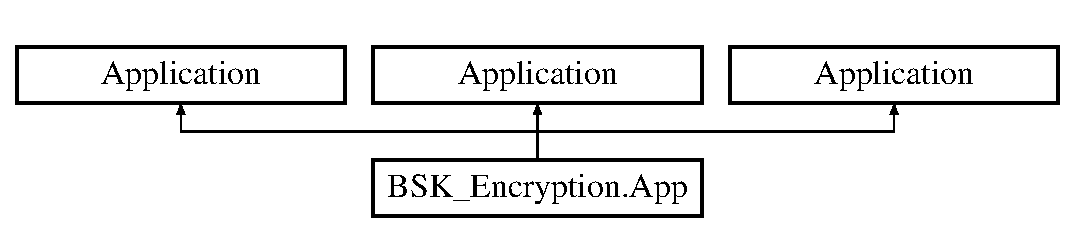
\includegraphics[height=2.000000cm]{class_b_s_k___encryption_1_1_app}
\end{center}
\end{figure}
\subsection*{Public Member Functions}
\begin{DoxyCompactItemize}
\item 
void \mbox{\hyperlink{class_b_s_k___encryption_1_1_app_a0a8c21b54e3defaaeb83f7ff03549074}{Initialize\+Component}} ()
\begin{DoxyCompactList}\small\item\em Initialize\+Component \end{DoxyCompactList}\item 
void \mbox{\hyperlink{class_b_s_k___encryption_1_1_app_a0a8c21b54e3defaaeb83f7ff03549074}{Initialize\+Component}} ()
\begin{DoxyCompactList}\small\item\em Initialize\+Component \end{DoxyCompactList}\end{DoxyCompactItemize}
\subsection*{Static Public Member Functions}
\begin{DoxyCompactItemize}
\item 
static void \mbox{\hyperlink{class_b_s_k___encryption_1_1_app_a93bd4c8173c18bc4f08e342fce264162}{Main}} ()
\begin{DoxyCompactList}\small\item\em Application Entry Point. \end{DoxyCompactList}\item 
static void \mbox{\hyperlink{class_b_s_k___encryption_1_1_app_a93bd4c8173c18bc4f08e342fce264162}{Main}} ()
\begin{DoxyCompactList}\small\item\em Application Entry Point. \end{DoxyCompactList}\end{DoxyCompactItemize}


\subsection{Detailed Description}
Interaction logic for App.\+xaml 

\mbox{\hyperlink{class_b_s_k___encryption_1_1_app}{App}} 

\subsection{Member Function Documentation}
\mbox{\Hypertarget{class_b_s_k___encryption_1_1_app_a0a8c21b54e3defaaeb83f7ff03549074}\label{class_b_s_k___encryption_1_1_app_a0a8c21b54e3defaaeb83f7ff03549074}} 
\index{B\+S\+K\+\_\+\+Encryption\+::\+App@{B\+S\+K\+\_\+\+Encryption\+::\+App}!Initialize\+Component@{Initialize\+Component}}
\index{Initialize\+Component@{Initialize\+Component}!B\+S\+K\+\_\+\+Encryption\+::\+App@{B\+S\+K\+\_\+\+Encryption\+::\+App}}
\subsubsection{\texorpdfstring{Initialize\+Component()}{InitializeComponent()}\hspace{0.1cm}{\footnotesize\ttfamily [1/2]}}
{\footnotesize\ttfamily void B\+S\+K\+\_\+\+Encryption.\+App.\+Initialize\+Component (\begin{DoxyParamCaption}{ }\end{DoxyParamCaption})}



Initialize\+Component 

\mbox{\Hypertarget{class_b_s_k___encryption_1_1_app_a0a8c21b54e3defaaeb83f7ff03549074}\label{class_b_s_k___encryption_1_1_app_a0a8c21b54e3defaaeb83f7ff03549074}} 
\index{B\+S\+K\+\_\+\+Encryption\+::\+App@{B\+S\+K\+\_\+\+Encryption\+::\+App}!Initialize\+Component@{Initialize\+Component}}
\index{Initialize\+Component@{Initialize\+Component}!B\+S\+K\+\_\+\+Encryption\+::\+App@{B\+S\+K\+\_\+\+Encryption\+::\+App}}
\subsubsection{\texorpdfstring{Initialize\+Component()}{InitializeComponent()}\hspace{0.1cm}{\footnotesize\ttfamily [2/2]}}
{\footnotesize\ttfamily void B\+S\+K\+\_\+\+Encryption.\+App.\+Initialize\+Component (\begin{DoxyParamCaption}{ }\end{DoxyParamCaption})}



Initialize\+Component 

\mbox{\Hypertarget{class_b_s_k___encryption_1_1_app_a93bd4c8173c18bc4f08e342fce264162}\label{class_b_s_k___encryption_1_1_app_a93bd4c8173c18bc4f08e342fce264162}} 
\index{B\+S\+K\+\_\+\+Encryption\+::\+App@{B\+S\+K\+\_\+\+Encryption\+::\+App}!Main@{Main}}
\index{Main@{Main}!B\+S\+K\+\_\+\+Encryption\+::\+App@{B\+S\+K\+\_\+\+Encryption\+::\+App}}
\subsubsection{\texorpdfstring{Main()}{Main()}\hspace{0.1cm}{\footnotesize\ttfamily [1/2]}}
{\footnotesize\ttfamily static void B\+S\+K\+\_\+\+Encryption.\+App.\+Main (\begin{DoxyParamCaption}{ }\end{DoxyParamCaption})\hspace{0.3cm}{\ttfamily [static]}}



Application Entry Point. 

\mbox{\Hypertarget{class_b_s_k___encryption_1_1_app_a93bd4c8173c18bc4f08e342fce264162}\label{class_b_s_k___encryption_1_1_app_a93bd4c8173c18bc4f08e342fce264162}} 
\index{B\+S\+K\+\_\+\+Encryption\+::\+App@{B\+S\+K\+\_\+\+Encryption\+::\+App}!Main@{Main}}
\index{Main@{Main}!B\+S\+K\+\_\+\+Encryption\+::\+App@{B\+S\+K\+\_\+\+Encryption\+::\+App}}
\subsubsection{\texorpdfstring{Main()}{Main()}\hspace{0.1cm}{\footnotesize\ttfamily [2/2]}}
{\footnotesize\ttfamily static void B\+S\+K\+\_\+\+Encryption.\+App.\+Main (\begin{DoxyParamCaption}{ }\end{DoxyParamCaption})\hspace{0.3cm}{\ttfamily [static]}}



Application Entry Point. 



The documentation for this class was generated from the following files\+:\begin{DoxyCompactItemize}
\item 
B\+S\+K\+\_\+\+Encryption/App.\+xaml.\+cs\item 
B\+S\+K\+\_\+\+Encryption/obj/\+Debug/App.\+g.\+cs\item 
B\+S\+K\+\_\+\+Encryption/obj/\+Debug/App.\+g.\+i.\+cs\end{DoxyCompactItemize}

\hypertarget{class_b_s_k___encryption_1_1_converters_1_1_block_converter}{}\section{B\+S\+K\+\_\+\+Encryption.\+Converters.\+Block\+Converter Class Reference}
\label{class_b_s_k___encryption_1_1_converters_1_1_block_converter}\index{B\+S\+K\+\_\+\+Encryption.\+Converters.\+Block\+Converter@{B\+S\+K\+\_\+\+Encryption.\+Converters.\+Block\+Converter}}


Converts int to string and back.  


Inheritance diagram for B\+S\+K\+\_\+\+Encryption.\+Converters.\+Block\+Converter\+:\begin{figure}[H]
\begin{center}
\leavevmode
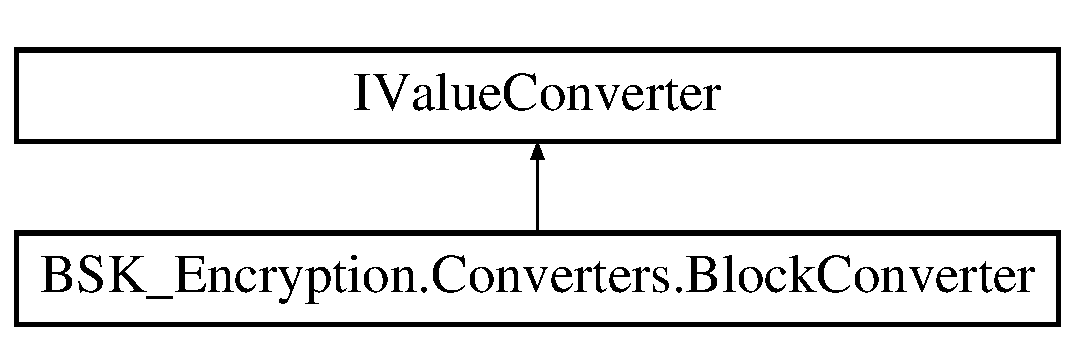
\includegraphics[height=2.000000cm]{class_b_s_k___encryption_1_1_converters_1_1_block_converter}
\end{center}
\end{figure}
\subsection*{Public Member Functions}
\begin{DoxyCompactItemize}
\item 
\mbox{\Hypertarget{class_b_s_k___encryption_1_1_converters_1_1_block_converter_a542b99e00c81b4a5af2e10bb7a32ae62}\label{class_b_s_k___encryption_1_1_converters_1_1_block_converter_a542b99e00c81b4a5af2e10bb7a32ae62}} 
object {\bfseries Convert} (object value, Type target\+Type, object parameter, Culture\+Info culture)
\item 
\mbox{\Hypertarget{class_b_s_k___encryption_1_1_converters_1_1_block_converter_a91fd1d884f9e81865130eabfaf62eebd}\label{class_b_s_k___encryption_1_1_converters_1_1_block_converter_a91fd1d884f9e81865130eabfaf62eebd}} 
object {\bfseries Convert\+Back} (object value, Type target\+Type, object parameter, Culture\+Info culture)
\end{DoxyCompactItemize}


\subsection{Detailed Description}
Converts int to string and back. 



The documentation for this class was generated from the following file\+:\begin{DoxyCompactItemize}
\item 
B\+S\+K\+\_\+\+Encryption/\+Converters/Block\+Converter.\+cs\end{DoxyCompactItemize}

\hypertarget{class_b_s_k___encryption_1_1_converters_1_1_cipher_converter}{}\section{B\+S\+K\+\_\+\+Encryption.\+Converters.\+Cipher\+Converter Class Reference}
\label{class_b_s_k___encryption_1_1_converters_1_1_cipher_converter}\index{B\+S\+K\+\_\+\+Encryption.\+Converters.\+Cipher\+Converter@{B\+S\+K\+\_\+\+Encryption.\+Converters.\+Cipher\+Converter}}


Converts to int from Cipher\+Mode and back.  


Inheritance diagram for B\+S\+K\+\_\+\+Encryption.\+Converters.\+Cipher\+Converter\+:\begin{figure}[H]
\begin{center}
\leavevmode
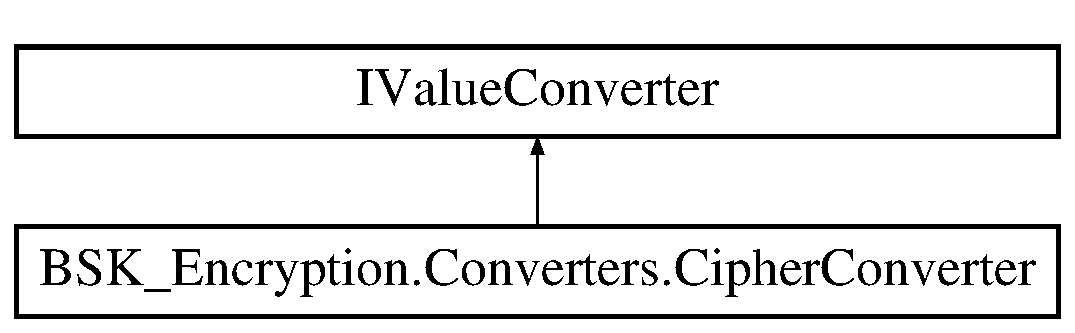
\includegraphics[height=2.000000cm]{class_b_s_k___encryption_1_1_converters_1_1_cipher_converter}
\end{center}
\end{figure}
\subsection*{Public Member Functions}
\begin{DoxyCompactItemize}
\item 
\mbox{\Hypertarget{class_b_s_k___encryption_1_1_converters_1_1_cipher_converter_a36010c8380c5fe2fa1285f745ce0f171}\label{class_b_s_k___encryption_1_1_converters_1_1_cipher_converter_a36010c8380c5fe2fa1285f745ce0f171}} 
object {\bfseries Convert} (object value, Type target\+Type, object parameter, Culture\+Info culture)
\item 
\mbox{\Hypertarget{class_b_s_k___encryption_1_1_converters_1_1_cipher_converter_aabade14f9218f1529b63e3c4c0cc0608}\label{class_b_s_k___encryption_1_1_converters_1_1_cipher_converter_aabade14f9218f1529b63e3c4c0cc0608}} 
object {\bfseries Convert\+Back} (object value, Type target\+Type, object parameter, Culture\+Info culture)
\end{DoxyCompactItemize}


\subsection{Detailed Description}
Converts to int from Cipher\+Mode and back. 



The documentation for this class was generated from the following file\+:\begin{DoxyCompactItemize}
\item 
B\+S\+K\+\_\+\+Encryption/\+Converters/Cipher\+Converter.\+cs\end{DoxyCompactItemize}

\hypertarget{class_b_s_k___encryption_1_1_view_models_1_1_data_view_model}{}\section{B\+S\+K\+\_\+\+Encryption.\+View\+Models.\+Data\+View\+Model Class Reference}
\label{class_b_s_k___encryption_1_1_view_models_1_1_data_view_model}\index{B\+S\+K\+\_\+\+Encryption.\+View\+Models.\+Data\+View\+Model@{B\+S\+K\+\_\+\+Encryption.\+View\+Models.\+Data\+View\+Model}}


Context for Cryptography.  


Inheritance diagram for B\+S\+K\+\_\+\+Encryption.\+View\+Models.\+Data\+View\+Model\+:\begin{figure}[H]
\begin{center}
\leavevmode
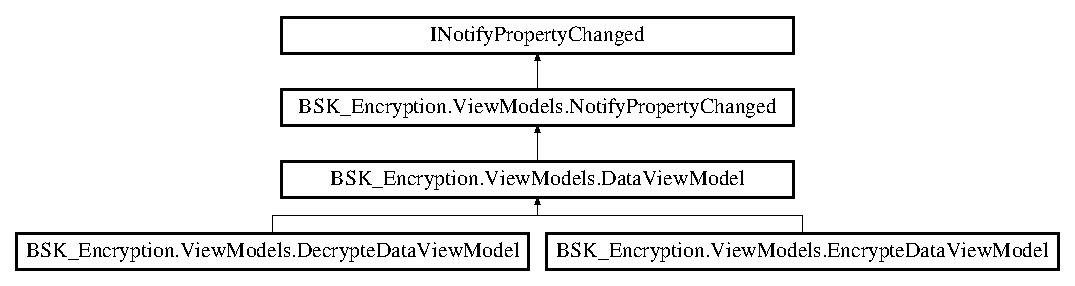
\includegraphics[height=3.393939cm]{class_b_s_k___encryption_1_1_view_models_1_1_data_view_model}
\end{center}
\end{figure}
\subsection*{Properties}
\begin{DoxyCompactItemize}
\item 
string \mbox{\hyperlink{class_b_s_k___encryption_1_1_view_models_1_1_data_view_model_a316ad59c641b9a8032095f33e9c76865}{Input\+Path}}\hspace{0.3cm}{\ttfamily  \mbox{[}get, set\mbox{]}}
\begin{DoxyCompactList}\small\item\em Input file path. \end{DoxyCompactList}\item 
string \mbox{\hyperlink{class_b_s_k___encryption_1_1_view_models_1_1_data_view_model_a1c4ad9bddae9ff3eb22e960c639e3382}{Output\+Path}}\hspace{0.3cm}{\ttfamily  \mbox{[}get, set\mbox{]}}
\begin{DoxyCompactList}\small\item\em Output file path. \end{DoxyCompactList}\item 
double \mbox{\hyperlink{class_b_s_k___encryption_1_1_view_models_1_1_data_view_model_a3473fbb812cdfe8a23b7f99c2e8db170}{Progress}}\hspace{0.3cm}{\ttfamily  \mbox{[}get, set\mbox{]}}
\begin{DoxyCompactList}\small\item\em Progress of cryptography operation. \end{DoxyCompactList}\item 
bool \mbox{\hyperlink{class_b_s_k___encryption_1_1_view_models_1_1_data_view_model_a2569f9d37164893d6201d52788d05742}{Is\+Not\+Running}}\hspace{0.3cm}{\ttfamily  \mbox{[}get, set\mbox{]}}
\begin{DoxyCompactList}\small\item\em Indicates if process is currently running. \end{DoxyCompactList}\end{DoxyCompactItemize}
\subsection*{Additional Inherited Members}


\subsection{Detailed Description}
Context for Cryptography. 



\subsection{Property Documentation}
\mbox{\Hypertarget{class_b_s_k___encryption_1_1_view_models_1_1_data_view_model_a316ad59c641b9a8032095f33e9c76865}\label{class_b_s_k___encryption_1_1_view_models_1_1_data_view_model_a316ad59c641b9a8032095f33e9c76865}} 
\index{B\+S\+K\+\_\+\+Encryption\+::\+View\+Models\+::\+Data\+View\+Model@{B\+S\+K\+\_\+\+Encryption\+::\+View\+Models\+::\+Data\+View\+Model}!Input\+Path@{Input\+Path}}
\index{Input\+Path@{Input\+Path}!B\+S\+K\+\_\+\+Encryption\+::\+View\+Models\+::\+Data\+View\+Model@{B\+S\+K\+\_\+\+Encryption\+::\+View\+Models\+::\+Data\+View\+Model}}
\subsubsection{\texorpdfstring{Input\+Path}{InputPath}}
{\footnotesize\ttfamily string B\+S\+K\+\_\+\+Encryption.\+View\+Models.\+Data\+View\+Model.\+Input\+Path\hspace{0.3cm}{\ttfamily [get]}, {\ttfamily [set]}}



Input file path. 

\mbox{\Hypertarget{class_b_s_k___encryption_1_1_view_models_1_1_data_view_model_a2569f9d37164893d6201d52788d05742}\label{class_b_s_k___encryption_1_1_view_models_1_1_data_view_model_a2569f9d37164893d6201d52788d05742}} 
\index{B\+S\+K\+\_\+\+Encryption\+::\+View\+Models\+::\+Data\+View\+Model@{B\+S\+K\+\_\+\+Encryption\+::\+View\+Models\+::\+Data\+View\+Model}!Is\+Not\+Running@{Is\+Not\+Running}}
\index{Is\+Not\+Running@{Is\+Not\+Running}!B\+S\+K\+\_\+\+Encryption\+::\+View\+Models\+::\+Data\+View\+Model@{B\+S\+K\+\_\+\+Encryption\+::\+View\+Models\+::\+Data\+View\+Model}}
\subsubsection{\texorpdfstring{Is\+Not\+Running}{IsNotRunning}}
{\footnotesize\ttfamily bool B\+S\+K\+\_\+\+Encryption.\+View\+Models.\+Data\+View\+Model.\+Is\+Not\+Running\hspace{0.3cm}{\ttfamily [get]}, {\ttfamily [set]}}



Indicates if process is currently running. 

\mbox{\Hypertarget{class_b_s_k___encryption_1_1_view_models_1_1_data_view_model_a1c4ad9bddae9ff3eb22e960c639e3382}\label{class_b_s_k___encryption_1_1_view_models_1_1_data_view_model_a1c4ad9bddae9ff3eb22e960c639e3382}} 
\index{B\+S\+K\+\_\+\+Encryption\+::\+View\+Models\+::\+Data\+View\+Model@{B\+S\+K\+\_\+\+Encryption\+::\+View\+Models\+::\+Data\+View\+Model}!Output\+Path@{Output\+Path}}
\index{Output\+Path@{Output\+Path}!B\+S\+K\+\_\+\+Encryption\+::\+View\+Models\+::\+Data\+View\+Model@{B\+S\+K\+\_\+\+Encryption\+::\+View\+Models\+::\+Data\+View\+Model}}
\subsubsection{\texorpdfstring{Output\+Path}{OutputPath}}
{\footnotesize\ttfamily string B\+S\+K\+\_\+\+Encryption.\+View\+Models.\+Data\+View\+Model.\+Output\+Path\hspace{0.3cm}{\ttfamily [get]}, {\ttfamily [set]}}



Output file path. 

\mbox{\Hypertarget{class_b_s_k___encryption_1_1_view_models_1_1_data_view_model_a3473fbb812cdfe8a23b7f99c2e8db170}\label{class_b_s_k___encryption_1_1_view_models_1_1_data_view_model_a3473fbb812cdfe8a23b7f99c2e8db170}} 
\index{B\+S\+K\+\_\+\+Encryption\+::\+View\+Models\+::\+Data\+View\+Model@{B\+S\+K\+\_\+\+Encryption\+::\+View\+Models\+::\+Data\+View\+Model}!Progress@{Progress}}
\index{Progress@{Progress}!B\+S\+K\+\_\+\+Encryption\+::\+View\+Models\+::\+Data\+View\+Model@{B\+S\+K\+\_\+\+Encryption\+::\+View\+Models\+::\+Data\+View\+Model}}
\subsubsection{\texorpdfstring{Progress}{Progress}}
{\footnotesize\ttfamily double B\+S\+K\+\_\+\+Encryption.\+View\+Models.\+Data\+View\+Model.\+Progress\hspace{0.3cm}{\ttfamily [get]}, {\ttfamily [set]}}



Progress of cryptography operation. 



The documentation for this class was generated from the following file\+:\begin{DoxyCompactItemize}
\item 
B\+S\+K\+\_\+\+Encryption/\+View\+Models/Data\+View\+Model.\+cs\end{DoxyCompactItemize}

\hypertarget{class_b_s_k___encryption_1_1_view_models_1_1_decrypte_data_view_model}{}\section{B\+S\+K\+\_\+\+Encryption.\+View\+Models.\+Decrypte\+Data\+View\+Model Class Reference}
\label{class_b_s_k___encryption_1_1_view_models_1_1_decrypte_data_view_model}\index{B\+S\+K\+\_\+\+Encryption.\+View\+Models.\+Decrypte\+Data\+View\+Model@{B\+S\+K\+\_\+\+Encryption.\+View\+Models.\+Decrypte\+Data\+View\+Model}}


Decrypt context model.  


Inheritance diagram for B\+S\+K\+\_\+\+Encryption.\+View\+Models.\+Decrypte\+Data\+View\+Model\+:\begin{figure}[H]
\begin{center}
\leavevmode
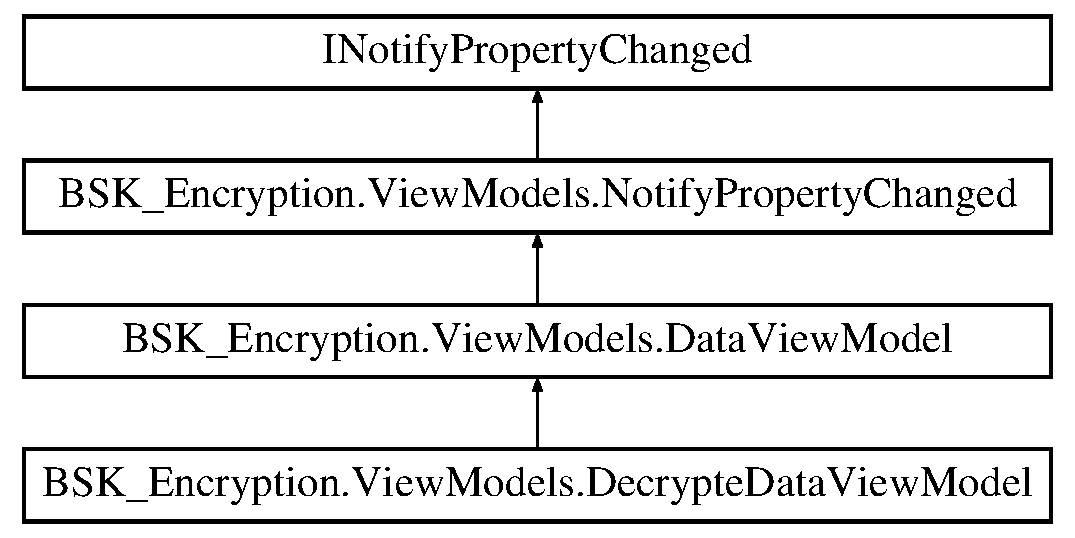
\includegraphics[height=4.000000cm]{class_b_s_k___encryption_1_1_view_models_1_1_decrypte_data_view_model}
\end{center}
\end{figure}
\subsection*{Properties}
\begin{DoxyCompactItemize}
\item 
string \mbox{\hyperlink{class_b_s_k___encryption_1_1_view_models_1_1_decrypte_data_view_model_ad5fdb1882096e5a0c7705c8112e7e6fa}{User}}\hspace{0.3cm}{\ttfamily  \mbox{[}get, set\mbox{]}}
\begin{DoxyCompactList}\small\item\em Username given from gui. \end{DoxyCompactList}\end{DoxyCompactItemize}
\subsection*{Additional Inherited Members}


\subsection{Detailed Description}
Decrypt context model. 



\subsection{Property Documentation}
\mbox{\Hypertarget{class_b_s_k___encryption_1_1_view_models_1_1_decrypte_data_view_model_ad5fdb1882096e5a0c7705c8112e7e6fa}\label{class_b_s_k___encryption_1_1_view_models_1_1_decrypte_data_view_model_ad5fdb1882096e5a0c7705c8112e7e6fa}} 
\index{B\+S\+K\+\_\+\+Encryption\+::\+View\+Models\+::\+Decrypte\+Data\+View\+Model@{B\+S\+K\+\_\+\+Encryption\+::\+View\+Models\+::\+Decrypte\+Data\+View\+Model}!User@{User}}
\index{User@{User}!B\+S\+K\+\_\+\+Encryption\+::\+View\+Models\+::\+Decrypte\+Data\+View\+Model@{B\+S\+K\+\_\+\+Encryption\+::\+View\+Models\+::\+Decrypte\+Data\+View\+Model}}
\subsubsection{\texorpdfstring{User}{User}}
{\footnotesize\ttfamily string B\+S\+K\+\_\+\+Encryption.\+View\+Models.\+Decrypte\+Data\+View\+Model.\+User\hspace{0.3cm}{\ttfamily [get]}, {\ttfamily [set]}}



Username given from gui. 



The documentation for this class was generated from the following file\+:\begin{DoxyCompactItemize}
\item 
B\+S\+K\+\_\+\+Encryption/\+View\+Models/Decrypte\+Data\+View\+Model.\+cs\end{DoxyCompactItemize}

\hypertarget{class_b_s_k___encryption_1_1_windows_1_1_decrypte_window}{}\section{B\+S\+K\+\_\+\+Encryption.\+Windows.\+Decrypte\+Window Class Reference}
\label{class_b_s_k___encryption_1_1_windows_1_1_decrypte_window}\index{B\+S\+K\+\_\+\+Encryption.\+Windows.\+Decrypte\+Window@{B\+S\+K\+\_\+\+Encryption.\+Windows.\+Decrypte\+Window}}


\mbox{\hyperlink{class_b_s_k___encryption_1_1_windows_1_1_decrypte_window}{Decrypte\+Window}}  


Inheritance diagram for B\+S\+K\+\_\+\+Encryption.\+Windows.\+Decrypte\+Window\+:\begin{figure}[H]
\begin{center}
\leavevmode
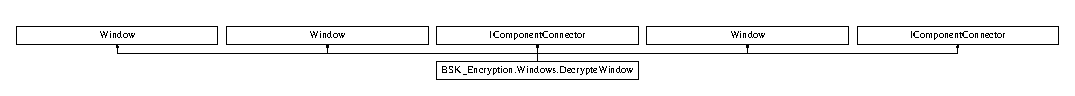
\includegraphics[height=0.842105cm]{class_b_s_k___encryption_1_1_windows_1_1_decrypte_window}
\end{center}
\end{figure}
\subsection*{Public Member Functions}
\begin{DoxyCompactItemize}
\item 
void \mbox{\hyperlink{class_b_s_k___encryption_1_1_windows_1_1_decrypte_window_aaec082894bb769855c76c4e67d541d71}{Initialize\+Component}} ()
\begin{DoxyCompactList}\small\item\em Initialize\+Component \end{DoxyCompactList}\item 
void \mbox{\hyperlink{class_b_s_k___encryption_1_1_windows_1_1_decrypte_window_aaec082894bb769855c76c4e67d541d71}{Initialize\+Component}} ()
\begin{DoxyCompactList}\small\item\em Initialize\+Component \end{DoxyCompactList}\end{DoxyCompactItemize}


\subsection{Detailed Description}
\mbox{\hyperlink{class_b_s_k___encryption_1_1_windows_1_1_decrypte_window}{Decrypte\+Window}} 

Interaction logic for Decrypte\+Window.\+xaml 

\subsection{Member Function Documentation}
\mbox{\Hypertarget{class_b_s_k___encryption_1_1_windows_1_1_decrypte_window_aaec082894bb769855c76c4e67d541d71}\label{class_b_s_k___encryption_1_1_windows_1_1_decrypte_window_aaec082894bb769855c76c4e67d541d71}} 
\index{B\+S\+K\+\_\+\+Encryption\+::\+Windows\+::\+Decrypte\+Window@{B\+S\+K\+\_\+\+Encryption\+::\+Windows\+::\+Decrypte\+Window}!Initialize\+Component@{Initialize\+Component}}
\index{Initialize\+Component@{Initialize\+Component}!B\+S\+K\+\_\+\+Encryption\+::\+Windows\+::\+Decrypte\+Window@{B\+S\+K\+\_\+\+Encryption\+::\+Windows\+::\+Decrypte\+Window}}
\subsubsection{\texorpdfstring{Initialize\+Component()}{InitializeComponent()}\hspace{0.1cm}{\footnotesize\ttfamily [1/2]}}
{\footnotesize\ttfamily void B\+S\+K\+\_\+\+Encryption.\+Windows.\+Decrypte\+Window.\+Initialize\+Component (\begin{DoxyParamCaption}{ }\end{DoxyParamCaption})}



Initialize\+Component 

\mbox{\Hypertarget{class_b_s_k___encryption_1_1_windows_1_1_decrypte_window_aaec082894bb769855c76c4e67d541d71}\label{class_b_s_k___encryption_1_1_windows_1_1_decrypte_window_aaec082894bb769855c76c4e67d541d71}} 
\index{B\+S\+K\+\_\+\+Encryption\+::\+Windows\+::\+Decrypte\+Window@{B\+S\+K\+\_\+\+Encryption\+::\+Windows\+::\+Decrypte\+Window}!Initialize\+Component@{Initialize\+Component}}
\index{Initialize\+Component@{Initialize\+Component}!B\+S\+K\+\_\+\+Encryption\+::\+Windows\+::\+Decrypte\+Window@{B\+S\+K\+\_\+\+Encryption\+::\+Windows\+::\+Decrypte\+Window}}
\subsubsection{\texorpdfstring{Initialize\+Component()}{InitializeComponent()}\hspace{0.1cm}{\footnotesize\ttfamily [2/2]}}
{\footnotesize\ttfamily void B\+S\+K\+\_\+\+Encryption.\+Windows.\+Decrypte\+Window.\+Initialize\+Component (\begin{DoxyParamCaption}{ }\end{DoxyParamCaption})}



Initialize\+Component 



The documentation for this class was generated from the following files\+:\begin{DoxyCompactItemize}
\item 
B\+S\+K\+\_\+\+Encryption/obj/\+Debug/\+Windows/Decrypte\+Window.\+g.\+cs\item 
B\+S\+K\+\_\+\+Encryption/obj/\+Debug/\+Windows/Decrypte\+Window.\+g.\+i.\+cs\item 
B\+S\+K\+\_\+\+Encryption/\+Windows/Decrypte\+Window.\+xaml.\+cs\end{DoxyCompactItemize}

\hypertarget{class_b_s_k___encryption_1_1_view_models_1_1_encrypte_data_view_model}{}\section{B\+S\+K\+\_\+\+Encryption.\+View\+Models.\+Encrypte\+Data\+View\+Model Class Reference}
\label{class_b_s_k___encryption_1_1_view_models_1_1_encrypte_data_view_model}\index{B\+S\+K\+\_\+\+Encryption.\+View\+Models.\+Encrypte\+Data\+View\+Model@{B\+S\+K\+\_\+\+Encryption.\+View\+Models.\+Encrypte\+Data\+View\+Model}}


Encrypt context model.  


Inheritance diagram for B\+S\+K\+\_\+\+Encryption.\+View\+Models.\+Encrypte\+Data\+View\+Model\+:\begin{figure}[H]
\begin{center}
\leavevmode
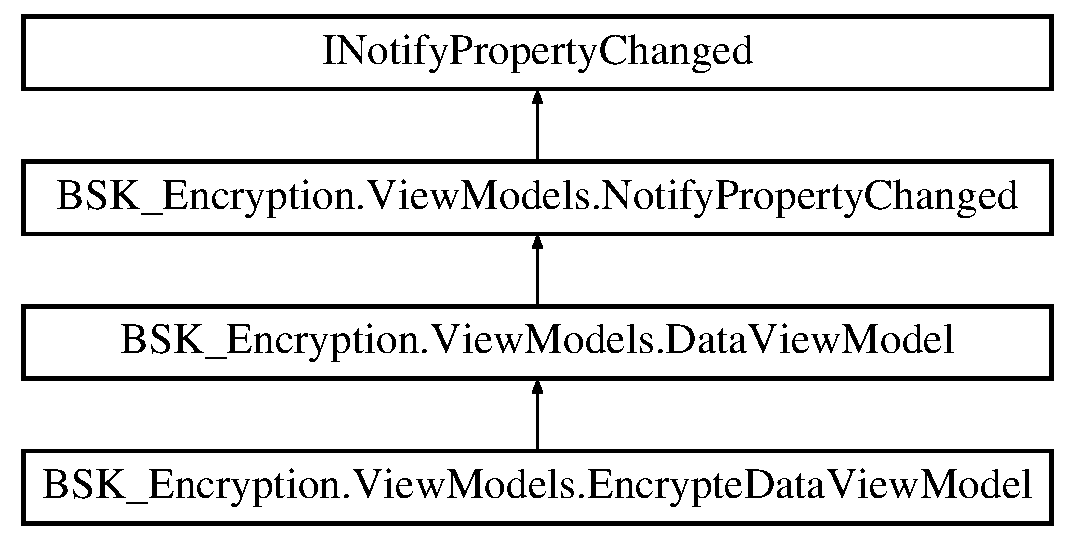
\includegraphics[height=4.000000cm]{class_b_s_k___encryption_1_1_view_models_1_1_encrypte_data_view_model}
\end{center}
\end{figure}
\subsection*{Properties}
\begin{DoxyCompactItemize}
\item 
Cipher\+Mode \mbox{\hyperlink{class_b_s_k___encryption_1_1_view_models_1_1_encrypte_data_view_model_a6f8281ab3e59382172dbc14fca178299}{Cipher}}\hspace{0.3cm}{\ttfamily  \mbox{[}get, set\mbox{]}}
\begin{DoxyCompactList}\small\item\em Type of given cipher from gui. \end{DoxyCompactList}\item 
int \mbox{\hyperlink{class_b_s_k___encryption_1_1_view_models_1_1_encrypte_data_view_model_a3740668ba5cb3c98ed43244ac8789e5f}{Key\+Size}}\hspace{0.3cm}{\ttfamily  \mbox{[}get, set\mbox{]}}
\begin{DoxyCompactList}\small\item\em Size of key given from gui. \end{DoxyCompactList}\item 
string \mbox{\hyperlink{class_b_s_k___encryption_1_1_view_models_1_1_encrypte_data_view_model_af8159eea8b1c4b4498db95f5d0cefa18}{User\+Names}}\hspace{0.3cm}{\ttfamily  \mbox{[}get\mbox{]}}
\begin{DoxyCompactList}\small\item\em Logins of users that will be authorized. Show only first 3 users. \end{DoxyCompactList}\item 
List$<$ string $>$ \mbox{\hyperlink{class_b_s_k___encryption_1_1_view_models_1_1_encrypte_data_view_model_ac7978e5838d18b867c66fa667bb5613e}{Users}}\hspace{0.3cm}{\ttfamily  \mbox{[}get, set\mbox{]}}
\begin{DoxyCompactList}\small\item\em List of users that will be authorized. \end{DoxyCompactList}\end{DoxyCompactItemize}
\subsection*{Additional Inherited Members}


\subsection{Detailed Description}
Encrypt context model. 



\subsection{Property Documentation}
\mbox{\Hypertarget{class_b_s_k___encryption_1_1_view_models_1_1_encrypte_data_view_model_a6f8281ab3e59382172dbc14fca178299}\label{class_b_s_k___encryption_1_1_view_models_1_1_encrypte_data_view_model_a6f8281ab3e59382172dbc14fca178299}} 
\index{B\+S\+K\+\_\+\+Encryption\+::\+View\+Models\+::\+Encrypte\+Data\+View\+Model@{B\+S\+K\+\_\+\+Encryption\+::\+View\+Models\+::\+Encrypte\+Data\+View\+Model}!Cipher@{Cipher}}
\index{Cipher@{Cipher}!B\+S\+K\+\_\+\+Encryption\+::\+View\+Models\+::\+Encrypte\+Data\+View\+Model@{B\+S\+K\+\_\+\+Encryption\+::\+View\+Models\+::\+Encrypte\+Data\+View\+Model}}
\subsubsection{\texorpdfstring{Cipher}{Cipher}}
{\footnotesize\ttfamily Cipher\+Mode B\+S\+K\+\_\+\+Encryption.\+View\+Models.\+Encrypte\+Data\+View\+Model.\+Cipher\hspace{0.3cm}{\ttfamily [get]}, {\ttfamily [set]}}



Type of given cipher from gui. 

\mbox{\Hypertarget{class_b_s_k___encryption_1_1_view_models_1_1_encrypte_data_view_model_a3740668ba5cb3c98ed43244ac8789e5f}\label{class_b_s_k___encryption_1_1_view_models_1_1_encrypte_data_view_model_a3740668ba5cb3c98ed43244ac8789e5f}} 
\index{B\+S\+K\+\_\+\+Encryption\+::\+View\+Models\+::\+Encrypte\+Data\+View\+Model@{B\+S\+K\+\_\+\+Encryption\+::\+View\+Models\+::\+Encrypte\+Data\+View\+Model}!Key\+Size@{Key\+Size}}
\index{Key\+Size@{Key\+Size}!B\+S\+K\+\_\+\+Encryption\+::\+View\+Models\+::\+Encrypte\+Data\+View\+Model@{B\+S\+K\+\_\+\+Encryption\+::\+View\+Models\+::\+Encrypte\+Data\+View\+Model}}
\subsubsection{\texorpdfstring{Key\+Size}{KeySize}}
{\footnotesize\ttfamily int B\+S\+K\+\_\+\+Encryption.\+View\+Models.\+Encrypte\+Data\+View\+Model.\+Key\+Size\hspace{0.3cm}{\ttfamily [get]}, {\ttfamily [set]}}



Size of key given from gui. 

\mbox{\Hypertarget{class_b_s_k___encryption_1_1_view_models_1_1_encrypte_data_view_model_af8159eea8b1c4b4498db95f5d0cefa18}\label{class_b_s_k___encryption_1_1_view_models_1_1_encrypte_data_view_model_af8159eea8b1c4b4498db95f5d0cefa18}} 
\index{B\+S\+K\+\_\+\+Encryption\+::\+View\+Models\+::\+Encrypte\+Data\+View\+Model@{B\+S\+K\+\_\+\+Encryption\+::\+View\+Models\+::\+Encrypte\+Data\+View\+Model}!User\+Names@{User\+Names}}
\index{User\+Names@{User\+Names}!B\+S\+K\+\_\+\+Encryption\+::\+View\+Models\+::\+Encrypte\+Data\+View\+Model@{B\+S\+K\+\_\+\+Encryption\+::\+View\+Models\+::\+Encrypte\+Data\+View\+Model}}
\subsubsection{\texorpdfstring{User\+Names}{UserNames}}
{\footnotesize\ttfamily string B\+S\+K\+\_\+\+Encryption.\+View\+Models.\+Encrypte\+Data\+View\+Model.\+User\+Names\hspace{0.3cm}{\ttfamily [get]}}



Logins of users that will be authorized. Show only first 3 users. 

\mbox{\Hypertarget{class_b_s_k___encryption_1_1_view_models_1_1_encrypte_data_view_model_ac7978e5838d18b867c66fa667bb5613e}\label{class_b_s_k___encryption_1_1_view_models_1_1_encrypte_data_view_model_ac7978e5838d18b867c66fa667bb5613e}} 
\index{B\+S\+K\+\_\+\+Encryption\+::\+View\+Models\+::\+Encrypte\+Data\+View\+Model@{B\+S\+K\+\_\+\+Encryption\+::\+View\+Models\+::\+Encrypte\+Data\+View\+Model}!Users@{Users}}
\index{Users@{Users}!B\+S\+K\+\_\+\+Encryption\+::\+View\+Models\+::\+Encrypte\+Data\+View\+Model@{B\+S\+K\+\_\+\+Encryption\+::\+View\+Models\+::\+Encrypte\+Data\+View\+Model}}
\subsubsection{\texorpdfstring{Users}{Users}}
{\footnotesize\ttfamily List$<$string$>$ B\+S\+K\+\_\+\+Encryption.\+View\+Models.\+Encrypte\+Data\+View\+Model.\+Users\hspace{0.3cm}{\ttfamily [get]}, {\ttfamily [set]}}



List of users that will be authorized. 



The documentation for this class was generated from the following file\+:\begin{DoxyCompactItemize}
\item 
B\+S\+K\+\_\+\+Encryption/\+View\+Models/Encrypte\+Data\+View\+Model.\+cs\end{DoxyCompactItemize}

\hypertarget{class_b_s_k___encryption_1_1_windows_1_1_encrypte_window}{}\section{B\+S\+K\+\_\+\+Encryption.\+Windows.\+Encrypte\+Window Class Reference}
\label{class_b_s_k___encryption_1_1_windows_1_1_encrypte_window}\index{B\+S\+K\+\_\+\+Encryption.\+Windows.\+Encrypte\+Window@{B\+S\+K\+\_\+\+Encryption.\+Windows.\+Encrypte\+Window}}


\mbox{\hyperlink{class_b_s_k___encryption_1_1_windows_1_1_encrypte_window}{Encrypte\+Window}}  


Inheritance diagram for B\+S\+K\+\_\+\+Encryption.\+Windows.\+Encrypte\+Window\+:\begin{figure}[H]
\begin{center}
\leavevmode
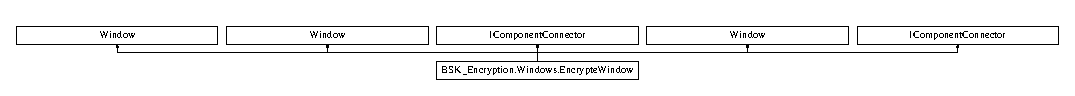
\includegraphics[height=0.845283cm]{class_b_s_k___encryption_1_1_windows_1_1_encrypte_window}
\end{center}
\end{figure}
\subsection*{Public Member Functions}
\begin{DoxyCompactItemize}
\item 
void \mbox{\hyperlink{class_b_s_k___encryption_1_1_windows_1_1_encrypte_window_a4d32979e0c636b65dbbdf621f64070d1}{Initialize\+Component}} ()
\begin{DoxyCompactList}\small\item\em Initialize\+Component \end{DoxyCompactList}\item 
void \mbox{\hyperlink{class_b_s_k___encryption_1_1_windows_1_1_encrypte_window_a4d32979e0c636b65dbbdf621f64070d1}{Initialize\+Component}} ()
\begin{DoxyCompactList}\small\item\em Initialize\+Component \end{DoxyCompactList}\end{DoxyCompactItemize}


\subsection{Detailed Description}
\mbox{\hyperlink{class_b_s_k___encryption_1_1_windows_1_1_encrypte_window}{Encrypte\+Window}} 

Interaction logic for Encrypte\+Window.\+xaml 

\subsection{Member Function Documentation}
\mbox{\Hypertarget{class_b_s_k___encryption_1_1_windows_1_1_encrypte_window_a4d32979e0c636b65dbbdf621f64070d1}\label{class_b_s_k___encryption_1_1_windows_1_1_encrypte_window_a4d32979e0c636b65dbbdf621f64070d1}} 
\index{B\+S\+K\+\_\+\+Encryption\+::\+Windows\+::\+Encrypte\+Window@{B\+S\+K\+\_\+\+Encryption\+::\+Windows\+::\+Encrypte\+Window}!Initialize\+Component@{Initialize\+Component}}
\index{Initialize\+Component@{Initialize\+Component}!B\+S\+K\+\_\+\+Encryption\+::\+Windows\+::\+Encrypte\+Window@{B\+S\+K\+\_\+\+Encryption\+::\+Windows\+::\+Encrypte\+Window}}
\subsubsection{\texorpdfstring{Initialize\+Component()}{InitializeComponent()}\hspace{0.1cm}{\footnotesize\ttfamily [1/2]}}
{\footnotesize\ttfamily void B\+S\+K\+\_\+\+Encryption.\+Windows.\+Encrypte\+Window.\+Initialize\+Component (\begin{DoxyParamCaption}{ }\end{DoxyParamCaption})}



Initialize\+Component 

\mbox{\Hypertarget{class_b_s_k___encryption_1_1_windows_1_1_encrypte_window_a4d32979e0c636b65dbbdf621f64070d1}\label{class_b_s_k___encryption_1_1_windows_1_1_encrypte_window_a4d32979e0c636b65dbbdf621f64070d1}} 
\index{B\+S\+K\+\_\+\+Encryption\+::\+Windows\+::\+Encrypte\+Window@{B\+S\+K\+\_\+\+Encryption\+::\+Windows\+::\+Encrypte\+Window}!Initialize\+Component@{Initialize\+Component}}
\index{Initialize\+Component@{Initialize\+Component}!B\+S\+K\+\_\+\+Encryption\+::\+Windows\+::\+Encrypte\+Window@{B\+S\+K\+\_\+\+Encryption\+::\+Windows\+::\+Encrypte\+Window}}
\subsubsection{\texorpdfstring{Initialize\+Component()}{InitializeComponent()}\hspace{0.1cm}{\footnotesize\ttfamily [2/2]}}
{\footnotesize\ttfamily void B\+S\+K\+\_\+\+Encryption.\+Windows.\+Encrypte\+Window.\+Initialize\+Component (\begin{DoxyParamCaption}{ }\end{DoxyParamCaption})}



Initialize\+Component 



The documentation for this class was generated from the following files\+:\begin{DoxyCompactItemize}
\item 
B\+S\+K\+\_\+\+Encryption/obj/\+Debug/\+Windows/Encrypte\+Window.\+g.\+cs\item 
B\+S\+K\+\_\+\+Encryption/obj/\+Debug/\+Windows/Encrypte\+Window.\+g.\+i.\+cs\item 
B\+S\+K\+\_\+\+Encryption/\+Windows/Encrypte\+Window.\+xaml.\+cs\end{DoxyCompactItemize}

\hypertarget{class_xaml_generated_namespace_1_1_generated_internal_type_helper}{}\section{Xaml\+Generated\+Namespace.\+Generated\+Internal\+Type\+Helper Class Reference}
\label{class_xaml_generated_namespace_1_1_generated_internal_type_helper}\index{Xaml\+Generated\+Namespace.\+Generated\+Internal\+Type\+Helper@{Xaml\+Generated\+Namespace.\+Generated\+Internal\+Type\+Helper}}


\mbox{\hyperlink{class_xaml_generated_namespace_1_1_generated_internal_type_helper}{Generated\+Internal\+Type\+Helper}}  


Inheritance diagram for Xaml\+Generated\+Namespace.\+Generated\+Internal\+Type\+Helper\+:\begin{figure}[H]
\begin{center}
\leavevmode
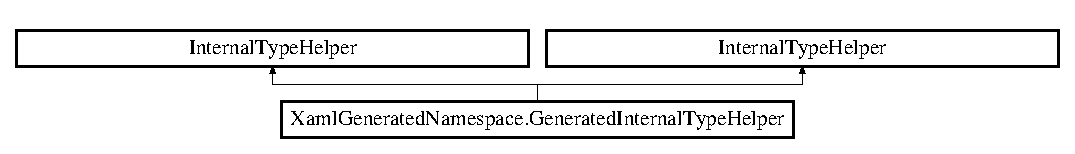
\includegraphics[height=1.627907cm]{class_xaml_generated_namespace_1_1_generated_internal_type_helper}
\end{center}
\end{figure}
\subsection*{Protected Member Functions}
\begin{DoxyCompactItemize}
\item 
override object \mbox{\hyperlink{class_xaml_generated_namespace_1_1_generated_internal_type_helper_aefb7a98fceb9c287cef4756942f441d1}{Create\+Instance}} (System.\+Type type, System.\+Globalization.\+Culture\+Info culture)
\begin{DoxyCompactList}\small\item\em Create\+Instance \end{DoxyCompactList}\item 
override object \mbox{\hyperlink{class_xaml_generated_namespace_1_1_generated_internal_type_helper_afdc9fe15b56607d02082908d934480c6}{Get\+Property\+Value}} (System.\+Reflection.\+Property\+Info property\+Info, object target, System.\+Globalization.\+Culture\+Info culture)
\begin{DoxyCompactList}\small\item\em Get\+Property\+Value \end{DoxyCompactList}\item 
override void \mbox{\hyperlink{class_xaml_generated_namespace_1_1_generated_internal_type_helper_ade0f04c0f7b18dd5b170e071d5534d38}{Set\+Property\+Value}} (System.\+Reflection.\+Property\+Info property\+Info, object target, object value, System.\+Globalization.\+Culture\+Info culture)
\begin{DoxyCompactList}\small\item\em Set\+Property\+Value \end{DoxyCompactList}\item 
override System.\+Delegate \mbox{\hyperlink{class_xaml_generated_namespace_1_1_generated_internal_type_helper_a8ec4c37e82d9f4e867e9655f4eac3a78}{Create\+Delegate}} (System.\+Type delegate\+Type, object target, string handler)
\begin{DoxyCompactList}\small\item\em Create\+Delegate \end{DoxyCompactList}\item 
override void \mbox{\hyperlink{class_xaml_generated_namespace_1_1_generated_internal_type_helper_a73471f4a6d1ca4c4fceec9ad8610f0c8}{Add\+Event\+Handler}} (System.\+Reflection.\+Event\+Info event\+Info, object target, System.\+Delegate handler)
\begin{DoxyCompactList}\small\item\em Add\+Event\+Handler \end{DoxyCompactList}\item 
override object \mbox{\hyperlink{class_xaml_generated_namespace_1_1_generated_internal_type_helper_aefb7a98fceb9c287cef4756942f441d1}{Create\+Instance}} (System.\+Type type, System.\+Globalization.\+Culture\+Info culture)
\begin{DoxyCompactList}\small\item\em Create\+Instance \end{DoxyCompactList}\item 
override object \mbox{\hyperlink{class_xaml_generated_namespace_1_1_generated_internal_type_helper_afdc9fe15b56607d02082908d934480c6}{Get\+Property\+Value}} (System.\+Reflection.\+Property\+Info property\+Info, object target, System.\+Globalization.\+Culture\+Info culture)
\begin{DoxyCompactList}\small\item\em Get\+Property\+Value \end{DoxyCompactList}\item 
override void \mbox{\hyperlink{class_xaml_generated_namespace_1_1_generated_internal_type_helper_ade0f04c0f7b18dd5b170e071d5534d38}{Set\+Property\+Value}} (System.\+Reflection.\+Property\+Info property\+Info, object target, object value, System.\+Globalization.\+Culture\+Info culture)
\begin{DoxyCompactList}\small\item\em Set\+Property\+Value \end{DoxyCompactList}\item 
override System.\+Delegate \mbox{\hyperlink{class_xaml_generated_namespace_1_1_generated_internal_type_helper_a8ec4c37e82d9f4e867e9655f4eac3a78}{Create\+Delegate}} (System.\+Type delegate\+Type, object target, string handler)
\begin{DoxyCompactList}\small\item\em Create\+Delegate \end{DoxyCompactList}\item 
override void \mbox{\hyperlink{class_xaml_generated_namespace_1_1_generated_internal_type_helper_a73471f4a6d1ca4c4fceec9ad8610f0c8}{Add\+Event\+Handler}} (System.\+Reflection.\+Event\+Info event\+Info, object target, System.\+Delegate handler)
\begin{DoxyCompactList}\small\item\em Add\+Event\+Handler \end{DoxyCompactList}\end{DoxyCompactItemize}


\subsection{Detailed Description}
\mbox{\hyperlink{class_xaml_generated_namespace_1_1_generated_internal_type_helper}{Generated\+Internal\+Type\+Helper}} 



\subsection{Member Function Documentation}
\mbox{\Hypertarget{class_xaml_generated_namespace_1_1_generated_internal_type_helper_a73471f4a6d1ca4c4fceec9ad8610f0c8}\label{class_xaml_generated_namespace_1_1_generated_internal_type_helper_a73471f4a6d1ca4c4fceec9ad8610f0c8}} 
\index{Xaml\+Generated\+Namespace\+::\+Generated\+Internal\+Type\+Helper@{Xaml\+Generated\+Namespace\+::\+Generated\+Internal\+Type\+Helper}!Add\+Event\+Handler@{Add\+Event\+Handler}}
\index{Add\+Event\+Handler@{Add\+Event\+Handler}!Xaml\+Generated\+Namespace\+::\+Generated\+Internal\+Type\+Helper@{Xaml\+Generated\+Namespace\+::\+Generated\+Internal\+Type\+Helper}}
\subsubsection{\texorpdfstring{Add\+Event\+Handler()}{AddEventHandler()}\hspace{0.1cm}{\footnotesize\ttfamily [1/2]}}
{\footnotesize\ttfamily override void Xaml\+Generated\+Namespace.\+Generated\+Internal\+Type\+Helper.\+Add\+Event\+Handler (\begin{DoxyParamCaption}\item[{System.\+Reflection.\+Event\+Info}]{event\+Info,  }\item[{object}]{target,  }\item[{System.\+Delegate}]{handler }\end{DoxyParamCaption})\hspace{0.3cm}{\ttfamily [protected]}}



Add\+Event\+Handler 

\mbox{\Hypertarget{class_xaml_generated_namespace_1_1_generated_internal_type_helper_a73471f4a6d1ca4c4fceec9ad8610f0c8}\label{class_xaml_generated_namespace_1_1_generated_internal_type_helper_a73471f4a6d1ca4c4fceec9ad8610f0c8}} 
\index{Xaml\+Generated\+Namespace\+::\+Generated\+Internal\+Type\+Helper@{Xaml\+Generated\+Namespace\+::\+Generated\+Internal\+Type\+Helper}!Add\+Event\+Handler@{Add\+Event\+Handler}}
\index{Add\+Event\+Handler@{Add\+Event\+Handler}!Xaml\+Generated\+Namespace\+::\+Generated\+Internal\+Type\+Helper@{Xaml\+Generated\+Namespace\+::\+Generated\+Internal\+Type\+Helper}}
\subsubsection{\texorpdfstring{Add\+Event\+Handler()}{AddEventHandler()}\hspace{0.1cm}{\footnotesize\ttfamily [2/2]}}
{\footnotesize\ttfamily override void Xaml\+Generated\+Namespace.\+Generated\+Internal\+Type\+Helper.\+Add\+Event\+Handler (\begin{DoxyParamCaption}\item[{System.\+Reflection.\+Event\+Info}]{event\+Info,  }\item[{object}]{target,  }\item[{System.\+Delegate}]{handler }\end{DoxyParamCaption})\hspace{0.3cm}{\ttfamily [protected]}}



Add\+Event\+Handler 

\mbox{\Hypertarget{class_xaml_generated_namespace_1_1_generated_internal_type_helper_a8ec4c37e82d9f4e867e9655f4eac3a78}\label{class_xaml_generated_namespace_1_1_generated_internal_type_helper_a8ec4c37e82d9f4e867e9655f4eac3a78}} 
\index{Xaml\+Generated\+Namespace\+::\+Generated\+Internal\+Type\+Helper@{Xaml\+Generated\+Namespace\+::\+Generated\+Internal\+Type\+Helper}!Create\+Delegate@{Create\+Delegate}}
\index{Create\+Delegate@{Create\+Delegate}!Xaml\+Generated\+Namespace\+::\+Generated\+Internal\+Type\+Helper@{Xaml\+Generated\+Namespace\+::\+Generated\+Internal\+Type\+Helper}}
\subsubsection{\texorpdfstring{Create\+Delegate()}{CreateDelegate()}\hspace{0.1cm}{\footnotesize\ttfamily [1/2]}}
{\footnotesize\ttfamily override System.\+Delegate Xaml\+Generated\+Namespace.\+Generated\+Internal\+Type\+Helper.\+Create\+Delegate (\begin{DoxyParamCaption}\item[{System.\+Type}]{delegate\+Type,  }\item[{object}]{target,  }\item[{string}]{handler }\end{DoxyParamCaption})\hspace{0.3cm}{\ttfamily [protected]}}



Create\+Delegate 

\mbox{\Hypertarget{class_xaml_generated_namespace_1_1_generated_internal_type_helper_a8ec4c37e82d9f4e867e9655f4eac3a78}\label{class_xaml_generated_namespace_1_1_generated_internal_type_helper_a8ec4c37e82d9f4e867e9655f4eac3a78}} 
\index{Xaml\+Generated\+Namespace\+::\+Generated\+Internal\+Type\+Helper@{Xaml\+Generated\+Namespace\+::\+Generated\+Internal\+Type\+Helper}!Create\+Delegate@{Create\+Delegate}}
\index{Create\+Delegate@{Create\+Delegate}!Xaml\+Generated\+Namespace\+::\+Generated\+Internal\+Type\+Helper@{Xaml\+Generated\+Namespace\+::\+Generated\+Internal\+Type\+Helper}}
\subsubsection{\texorpdfstring{Create\+Delegate()}{CreateDelegate()}\hspace{0.1cm}{\footnotesize\ttfamily [2/2]}}
{\footnotesize\ttfamily override System.\+Delegate Xaml\+Generated\+Namespace.\+Generated\+Internal\+Type\+Helper.\+Create\+Delegate (\begin{DoxyParamCaption}\item[{System.\+Type}]{delegate\+Type,  }\item[{object}]{target,  }\item[{string}]{handler }\end{DoxyParamCaption})\hspace{0.3cm}{\ttfamily [protected]}}



Create\+Delegate 

\mbox{\Hypertarget{class_xaml_generated_namespace_1_1_generated_internal_type_helper_aefb7a98fceb9c287cef4756942f441d1}\label{class_xaml_generated_namespace_1_1_generated_internal_type_helper_aefb7a98fceb9c287cef4756942f441d1}} 
\index{Xaml\+Generated\+Namespace\+::\+Generated\+Internal\+Type\+Helper@{Xaml\+Generated\+Namespace\+::\+Generated\+Internal\+Type\+Helper}!Create\+Instance@{Create\+Instance}}
\index{Create\+Instance@{Create\+Instance}!Xaml\+Generated\+Namespace\+::\+Generated\+Internal\+Type\+Helper@{Xaml\+Generated\+Namespace\+::\+Generated\+Internal\+Type\+Helper}}
\subsubsection{\texorpdfstring{Create\+Instance()}{CreateInstance()}\hspace{0.1cm}{\footnotesize\ttfamily [1/2]}}
{\footnotesize\ttfamily override object Xaml\+Generated\+Namespace.\+Generated\+Internal\+Type\+Helper.\+Create\+Instance (\begin{DoxyParamCaption}\item[{System.\+Type}]{type,  }\item[{System.\+Globalization.\+Culture\+Info}]{culture }\end{DoxyParamCaption})\hspace{0.3cm}{\ttfamily [protected]}}



Create\+Instance 

\mbox{\Hypertarget{class_xaml_generated_namespace_1_1_generated_internal_type_helper_aefb7a98fceb9c287cef4756942f441d1}\label{class_xaml_generated_namespace_1_1_generated_internal_type_helper_aefb7a98fceb9c287cef4756942f441d1}} 
\index{Xaml\+Generated\+Namespace\+::\+Generated\+Internal\+Type\+Helper@{Xaml\+Generated\+Namespace\+::\+Generated\+Internal\+Type\+Helper}!Create\+Instance@{Create\+Instance}}
\index{Create\+Instance@{Create\+Instance}!Xaml\+Generated\+Namespace\+::\+Generated\+Internal\+Type\+Helper@{Xaml\+Generated\+Namespace\+::\+Generated\+Internal\+Type\+Helper}}
\subsubsection{\texorpdfstring{Create\+Instance()}{CreateInstance()}\hspace{0.1cm}{\footnotesize\ttfamily [2/2]}}
{\footnotesize\ttfamily override object Xaml\+Generated\+Namespace.\+Generated\+Internal\+Type\+Helper.\+Create\+Instance (\begin{DoxyParamCaption}\item[{System.\+Type}]{type,  }\item[{System.\+Globalization.\+Culture\+Info}]{culture }\end{DoxyParamCaption})\hspace{0.3cm}{\ttfamily [protected]}}



Create\+Instance 

\mbox{\Hypertarget{class_xaml_generated_namespace_1_1_generated_internal_type_helper_afdc9fe15b56607d02082908d934480c6}\label{class_xaml_generated_namespace_1_1_generated_internal_type_helper_afdc9fe15b56607d02082908d934480c6}} 
\index{Xaml\+Generated\+Namespace\+::\+Generated\+Internal\+Type\+Helper@{Xaml\+Generated\+Namespace\+::\+Generated\+Internal\+Type\+Helper}!Get\+Property\+Value@{Get\+Property\+Value}}
\index{Get\+Property\+Value@{Get\+Property\+Value}!Xaml\+Generated\+Namespace\+::\+Generated\+Internal\+Type\+Helper@{Xaml\+Generated\+Namespace\+::\+Generated\+Internal\+Type\+Helper}}
\subsubsection{\texorpdfstring{Get\+Property\+Value()}{GetPropertyValue()}\hspace{0.1cm}{\footnotesize\ttfamily [1/2]}}
{\footnotesize\ttfamily override object Xaml\+Generated\+Namespace.\+Generated\+Internal\+Type\+Helper.\+Get\+Property\+Value (\begin{DoxyParamCaption}\item[{System.\+Reflection.\+Property\+Info}]{property\+Info,  }\item[{object}]{target,  }\item[{System.\+Globalization.\+Culture\+Info}]{culture }\end{DoxyParamCaption})\hspace{0.3cm}{\ttfamily [protected]}}



Get\+Property\+Value 

\mbox{\Hypertarget{class_xaml_generated_namespace_1_1_generated_internal_type_helper_afdc9fe15b56607d02082908d934480c6}\label{class_xaml_generated_namespace_1_1_generated_internal_type_helper_afdc9fe15b56607d02082908d934480c6}} 
\index{Xaml\+Generated\+Namespace\+::\+Generated\+Internal\+Type\+Helper@{Xaml\+Generated\+Namespace\+::\+Generated\+Internal\+Type\+Helper}!Get\+Property\+Value@{Get\+Property\+Value}}
\index{Get\+Property\+Value@{Get\+Property\+Value}!Xaml\+Generated\+Namespace\+::\+Generated\+Internal\+Type\+Helper@{Xaml\+Generated\+Namespace\+::\+Generated\+Internal\+Type\+Helper}}
\subsubsection{\texorpdfstring{Get\+Property\+Value()}{GetPropertyValue()}\hspace{0.1cm}{\footnotesize\ttfamily [2/2]}}
{\footnotesize\ttfamily override object Xaml\+Generated\+Namespace.\+Generated\+Internal\+Type\+Helper.\+Get\+Property\+Value (\begin{DoxyParamCaption}\item[{System.\+Reflection.\+Property\+Info}]{property\+Info,  }\item[{object}]{target,  }\item[{System.\+Globalization.\+Culture\+Info}]{culture }\end{DoxyParamCaption})\hspace{0.3cm}{\ttfamily [protected]}}



Get\+Property\+Value 

\mbox{\Hypertarget{class_xaml_generated_namespace_1_1_generated_internal_type_helper_ade0f04c0f7b18dd5b170e071d5534d38}\label{class_xaml_generated_namespace_1_1_generated_internal_type_helper_ade0f04c0f7b18dd5b170e071d5534d38}} 
\index{Xaml\+Generated\+Namespace\+::\+Generated\+Internal\+Type\+Helper@{Xaml\+Generated\+Namespace\+::\+Generated\+Internal\+Type\+Helper}!Set\+Property\+Value@{Set\+Property\+Value}}
\index{Set\+Property\+Value@{Set\+Property\+Value}!Xaml\+Generated\+Namespace\+::\+Generated\+Internal\+Type\+Helper@{Xaml\+Generated\+Namespace\+::\+Generated\+Internal\+Type\+Helper}}
\subsubsection{\texorpdfstring{Set\+Property\+Value()}{SetPropertyValue()}\hspace{0.1cm}{\footnotesize\ttfamily [1/2]}}
{\footnotesize\ttfamily override void Xaml\+Generated\+Namespace.\+Generated\+Internal\+Type\+Helper.\+Set\+Property\+Value (\begin{DoxyParamCaption}\item[{System.\+Reflection.\+Property\+Info}]{property\+Info,  }\item[{object}]{target,  }\item[{object}]{value,  }\item[{System.\+Globalization.\+Culture\+Info}]{culture }\end{DoxyParamCaption})\hspace{0.3cm}{\ttfamily [protected]}}



Set\+Property\+Value 

\mbox{\Hypertarget{class_xaml_generated_namespace_1_1_generated_internal_type_helper_ade0f04c0f7b18dd5b170e071d5534d38}\label{class_xaml_generated_namespace_1_1_generated_internal_type_helper_ade0f04c0f7b18dd5b170e071d5534d38}} 
\index{Xaml\+Generated\+Namespace\+::\+Generated\+Internal\+Type\+Helper@{Xaml\+Generated\+Namespace\+::\+Generated\+Internal\+Type\+Helper}!Set\+Property\+Value@{Set\+Property\+Value}}
\index{Set\+Property\+Value@{Set\+Property\+Value}!Xaml\+Generated\+Namespace\+::\+Generated\+Internal\+Type\+Helper@{Xaml\+Generated\+Namespace\+::\+Generated\+Internal\+Type\+Helper}}
\subsubsection{\texorpdfstring{Set\+Property\+Value()}{SetPropertyValue()}\hspace{0.1cm}{\footnotesize\ttfamily [2/2]}}
{\footnotesize\ttfamily override void Xaml\+Generated\+Namespace.\+Generated\+Internal\+Type\+Helper.\+Set\+Property\+Value (\begin{DoxyParamCaption}\item[{System.\+Reflection.\+Property\+Info}]{property\+Info,  }\item[{object}]{target,  }\item[{object}]{value,  }\item[{System.\+Globalization.\+Culture\+Info}]{culture }\end{DoxyParamCaption})\hspace{0.3cm}{\ttfamily [protected]}}



Set\+Property\+Value 



The documentation for this class was generated from the following files\+:\begin{DoxyCompactItemize}
\item 
B\+S\+K\+\_\+\+Encryption/obj/\+Debug/Generated\+Internal\+Type\+Helper.\+g.\+cs\item 
B\+S\+K\+\_\+\+Encryption/obj/\+Debug/Generated\+Internal\+Type\+Helper.\+g.\+i.\+cs\end{DoxyCompactItemize}

\hypertarget{class_b_s_k___encryption_1_1_validators_1_1_input_path_validator}{}\section{B\+S\+K\+\_\+\+Encryption.\+Validators.\+Input\+Path\+Validator Class Reference}
\label{class_b_s_k___encryption_1_1_validators_1_1_input_path_validator}\index{B\+S\+K\+\_\+\+Encryption.\+Validators.\+Input\+Path\+Validator@{B\+S\+K\+\_\+\+Encryption.\+Validators.\+Input\+Path\+Validator}}


Validator for path  


Inheritance diagram for B\+S\+K\+\_\+\+Encryption.\+Validators.\+Input\+Path\+Validator\+:\begin{figure}[H]
\begin{center}
\leavevmode
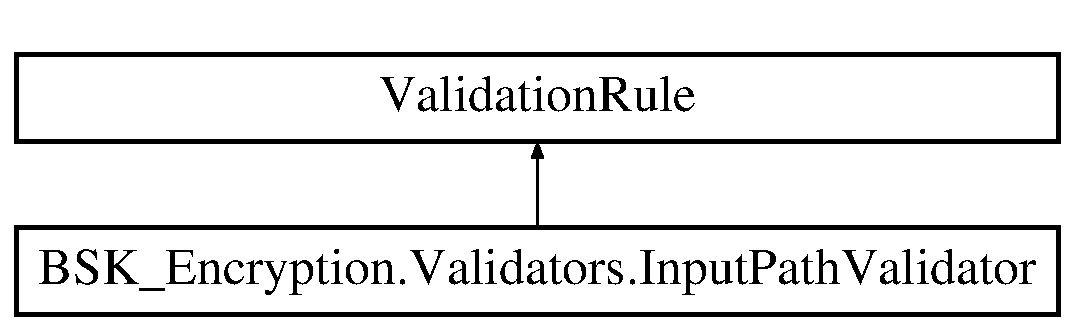
\includegraphics[height=2.000000cm]{class_b_s_k___encryption_1_1_validators_1_1_input_path_validator}
\end{center}
\end{figure}
\subsection*{Public Member Functions}
\begin{DoxyCompactItemize}
\item 
\mbox{\Hypertarget{class_b_s_k___encryption_1_1_validators_1_1_input_path_validator_a124786fbed1512ca70b2e54e90cdb7e4}\label{class_b_s_k___encryption_1_1_validators_1_1_input_path_validator_a124786fbed1512ca70b2e54e90cdb7e4}} 
override Validation\+Result {\bfseries Validate} (object value, Culture\+Info culture\+Info)
\end{DoxyCompactItemize}


\subsection{Detailed Description}
Validator for path 



The documentation for this class was generated from the following file\+:\begin{DoxyCompactItemize}
\item 
B\+S\+K\+\_\+\+Encryption/\+Validators/Input\+Path\+Validator.\+cs\end{DoxyCompactItemize}

\hypertarget{class_b_s_k___encryption_1_1_windows_1_1_main_window}{}\section{B\+S\+K\+\_\+\+Encryption.\+Windows.\+Main\+Window Class Reference}
\label{class_b_s_k___encryption_1_1_windows_1_1_main_window}\index{B\+S\+K\+\_\+\+Encryption.\+Windows.\+Main\+Window@{B\+S\+K\+\_\+\+Encryption.\+Windows.\+Main\+Window}}


\mbox{\hyperlink{class_b_s_k___encryption_1_1_windows_1_1_main_window}{Main\+Window}}  


Inheritance diagram for B\+S\+K\+\_\+\+Encryption.\+Windows.\+Main\+Window\+:\begin{figure}[H]
\begin{center}
\leavevmode
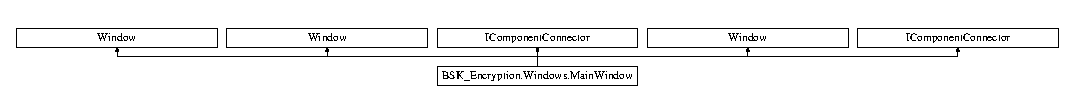
\includegraphics[height=0.925620cm]{class_b_s_k___encryption_1_1_windows_1_1_main_window}
\end{center}
\end{figure}
\subsection*{Public Member Functions}
\begin{DoxyCompactItemize}
\item 
void \mbox{\hyperlink{class_b_s_k___encryption_1_1_windows_1_1_main_window_ad2eaef015028e1367f97c86e7c9878da}{Initialize\+Component}} ()
\begin{DoxyCompactList}\small\item\em Initialize\+Component \end{DoxyCompactList}\item 
void \mbox{\hyperlink{class_b_s_k___encryption_1_1_windows_1_1_main_window_ad2eaef015028e1367f97c86e7c9878da}{Initialize\+Component}} ()
\begin{DoxyCompactList}\small\item\em Initialize\+Component \end{DoxyCompactList}\end{DoxyCompactItemize}


\subsection{Detailed Description}
\mbox{\hyperlink{class_b_s_k___encryption_1_1_windows_1_1_main_window}{Main\+Window}} 

Interaction logic for Main\+Window.\+xaml 

\subsection{Member Function Documentation}
\mbox{\Hypertarget{class_b_s_k___encryption_1_1_windows_1_1_main_window_ad2eaef015028e1367f97c86e7c9878da}\label{class_b_s_k___encryption_1_1_windows_1_1_main_window_ad2eaef015028e1367f97c86e7c9878da}} 
\index{B\+S\+K\+\_\+\+Encryption\+::\+Windows\+::\+Main\+Window@{B\+S\+K\+\_\+\+Encryption\+::\+Windows\+::\+Main\+Window}!Initialize\+Component@{Initialize\+Component}}
\index{Initialize\+Component@{Initialize\+Component}!B\+S\+K\+\_\+\+Encryption\+::\+Windows\+::\+Main\+Window@{B\+S\+K\+\_\+\+Encryption\+::\+Windows\+::\+Main\+Window}}
\subsubsection{\texorpdfstring{Initialize\+Component()}{InitializeComponent()}\hspace{0.1cm}{\footnotesize\ttfamily [1/2]}}
{\footnotesize\ttfamily void B\+S\+K\+\_\+\+Encryption.\+Windows.\+Main\+Window.\+Initialize\+Component (\begin{DoxyParamCaption}{ }\end{DoxyParamCaption})}



Initialize\+Component 

\mbox{\Hypertarget{class_b_s_k___encryption_1_1_windows_1_1_main_window_ad2eaef015028e1367f97c86e7c9878da}\label{class_b_s_k___encryption_1_1_windows_1_1_main_window_ad2eaef015028e1367f97c86e7c9878da}} 
\index{B\+S\+K\+\_\+\+Encryption\+::\+Windows\+::\+Main\+Window@{B\+S\+K\+\_\+\+Encryption\+::\+Windows\+::\+Main\+Window}!Initialize\+Component@{Initialize\+Component}}
\index{Initialize\+Component@{Initialize\+Component}!B\+S\+K\+\_\+\+Encryption\+::\+Windows\+::\+Main\+Window@{B\+S\+K\+\_\+\+Encryption\+::\+Windows\+::\+Main\+Window}}
\subsubsection{\texorpdfstring{Initialize\+Component()}{InitializeComponent()}\hspace{0.1cm}{\footnotesize\ttfamily [2/2]}}
{\footnotesize\ttfamily void B\+S\+K\+\_\+\+Encryption.\+Windows.\+Main\+Window.\+Initialize\+Component (\begin{DoxyParamCaption}{ }\end{DoxyParamCaption})}



Initialize\+Component 



The documentation for this class was generated from the following files\+:\begin{DoxyCompactItemize}
\item 
B\+S\+K\+\_\+\+Encryption/obj/\+Debug/\+Windows/Main\+Window.\+g.\+cs\item 
B\+S\+K\+\_\+\+Encryption/obj/\+Debug/\+Windows/Main\+Window.\+g.\+i.\+cs\item 
B\+S\+K\+\_\+\+Encryption/\+Windows/Main\+Window.\+xaml.\+cs\end{DoxyCompactItemize}

\hypertarget{class_b_s_k___encryption_1_1_view_models_1_1_notify_property_changed}{}\section{B\+S\+K\+\_\+\+Encryption.\+View\+Models.\+Notify\+Property\+Changed Class Reference}
\label{class_b_s_k___encryption_1_1_view_models_1_1_notify_property_changed}\index{B\+S\+K\+\_\+\+Encryption.\+View\+Models.\+Notify\+Property\+Changed@{B\+S\+K\+\_\+\+Encryption.\+View\+Models.\+Notify\+Property\+Changed}}
Inheritance diagram for B\+S\+K\+\_\+\+Encryption.\+View\+Models.\+Notify\+Property\+Changed\+:\begin{figure}[H]
\begin{center}
\leavevmode
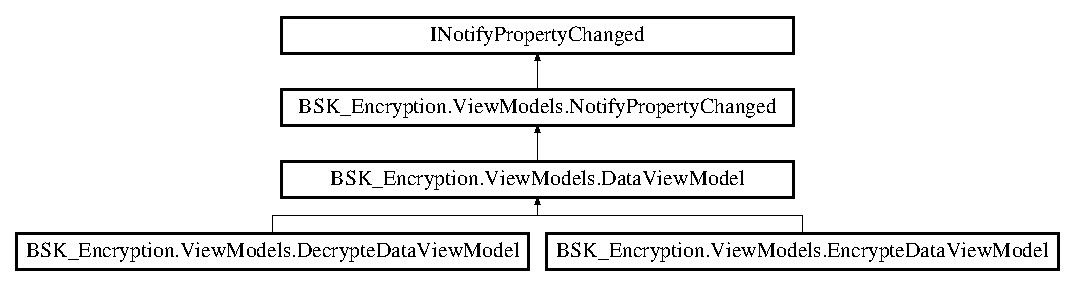
\includegraphics[height=3.393939cm]{class_b_s_k___encryption_1_1_view_models_1_1_notify_property_changed}
\end{center}
\end{figure}
\subsection*{Public Member Functions}
\begin{DoxyCompactItemize}
\item 
\mbox{\Hypertarget{class_b_s_k___encryption_1_1_view_models_1_1_notify_property_changed_afe474cbf0d45c9fefa3ead91095bac89}\label{class_b_s_k___encryption_1_1_view_models_1_1_notify_property_changed_afe474cbf0d45c9fefa3ead91095bac89}} 
void {\bfseries On\+Property\+Changed} (\mbox{[}Caller\+Member\+Name\mbox{]} string property\+Name=\char`\"{}\char`\"{})
\end{DoxyCompactItemize}
\subsection*{Events}
\begin{DoxyCompactItemize}
\item 
\mbox{\Hypertarget{class_b_s_k___encryption_1_1_view_models_1_1_notify_property_changed_a719ad354061f0bf6f3aaa4a5093fdb2f}\label{class_b_s_k___encryption_1_1_view_models_1_1_notify_property_changed_a719ad354061f0bf6f3aaa4a5093fdb2f}} 
Property\+Changed\+Event\+Handler {\bfseries Property\+Changed}
\end{DoxyCompactItemize}


The documentation for this class was generated from the following file\+:\begin{DoxyCompactItemize}
\item 
B\+S\+K\+\_\+\+Encryption/\+View\+Models/Notify\+Property\+Changed.\+cs\end{DoxyCompactItemize}

\hypertarget{class_b_s_k___encryption_1_1_encryption_1_1_o_f_b_1_1_o_f_b_stream}{}\section{B\+S\+K\+\_\+\+Encryption.\+Encryption.\+O\+F\+B.\+O\+F\+B\+Stream Class Reference}
\label{class_b_s_k___encryption_1_1_encryption_1_1_o_f_b_1_1_o_f_b_stream}\index{B\+S\+K\+\_\+\+Encryption.\+Encryption.\+O\+F\+B.\+O\+F\+B\+Stream@{B\+S\+K\+\_\+\+Encryption.\+Encryption.\+O\+F\+B.\+O\+F\+B\+Stream}}


Extension to the Rijandael\+Managed for using \mbox{\hyperlink{namespace_b_s_k___encryption_1_1_encryption_1_1_o_f_b}{O\+FB}} mode.  


Inheritance diagram for B\+S\+K\+\_\+\+Encryption.\+Encryption.\+O\+F\+B.\+O\+F\+B\+Stream\+:\begin{figure}[H]
\begin{center}
\leavevmode
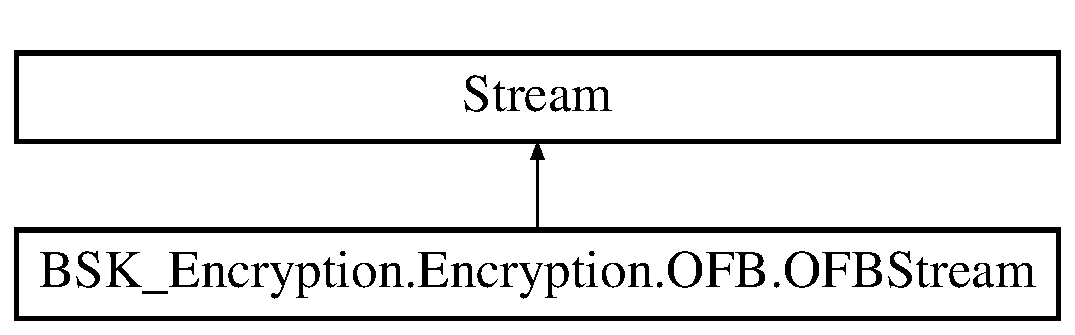
\includegraphics[height=2.000000cm]{class_b_s_k___encryption_1_1_encryption_1_1_o_f_b_1_1_o_f_b_stream}
\end{center}
\end{figure}
\subsection*{Public Member Functions}
\begin{DoxyCompactItemize}
\item 
\mbox{\hyperlink{class_b_s_k___encryption_1_1_encryption_1_1_o_f_b_1_1_o_f_b_stream_ad0ce9d5e1753dd3b01fd6c883f7c794a}{O\+F\+B\+Stream}} (Stream parent, Symmetric\+Algorithm algo, Crypto\+Stream\+Mode mode)
\begin{DoxyCompactList}\small\item\em Constructor for the extension stream. \end{DoxyCompactList}\item 
\mbox{\Hypertarget{class_b_s_k___encryption_1_1_encryption_1_1_o_f_b_1_1_o_f_b_stream_a69241ac77bb1f463519624c31aeae7c4}\label{class_b_s_k___encryption_1_1_encryption_1_1_o_f_b_1_1_o_f_b_stream_a69241ac77bb1f463519624c31aeae7c4}} 
override int {\bfseries Read} (byte\mbox{[}$\,$\mbox{]} buffer, int offset, int count)
\item 
\mbox{\Hypertarget{class_b_s_k___encryption_1_1_encryption_1_1_o_f_b_1_1_o_f_b_stream_a696a23586bf7ec0d4a60d98f8078f47d}\label{class_b_s_k___encryption_1_1_encryption_1_1_o_f_b_1_1_o_f_b_stream_a696a23586bf7ec0d4a60d98f8078f47d}} 
override void {\bfseries Write} (byte\mbox{[}$\,$\mbox{]} buffer, int offset, int count)
\item 
\mbox{\Hypertarget{class_b_s_k___encryption_1_1_encryption_1_1_o_f_b_1_1_o_f_b_stream_a69c8c165f3dd34f31c9fe799d5ca0553}\label{class_b_s_k___encryption_1_1_encryption_1_1_o_f_b_1_1_o_f_b_stream_a69c8c165f3dd34f31c9fe799d5ca0553}} 
override void {\bfseries Flush} ()
\item 
\mbox{\Hypertarget{class_b_s_k___encryption_1_1_encryption_1_1_o_f_b_1_1_o_f_b_stream_a1ddfc639f68b7da48e6b86922409213b}\label{class_b_s_k___encryption_1_1_encryption_1_1_o_f_b_1_1_o_f_b_stream_a1ddfc639f68b7da48e6b86922409213b}} 
override long {\bfseries Seek} (long offset, System.\+I\+O.\+Seek\+Origin origin)
\item 
\mbox{\Hypertarget{class_b_s_k___encryption_1_1_encryption_1_1_o_f_b_1_1_o_f_b_stream_a120e8bfecd3b9bd050088b397e4c3787}\label{class_b_s_k___encryption_1_1_encryption_1_1_o_f_b_1_1_o_f_b_stream_a120e8bfecd3b9bd050088b397e4c3787}} 
override void {\bfseries Set\+Length} (long value)
\end{DoxyCompactItemize}
\subsection*{Properties}
\begin{DoxyCompactItemize}
\item 
\mbox{\Hypertarget{class_b_s_k___encryption_1_1_encryption_1_1_o_f_b_1_1_o_f_b_stream_a3218b3890ff3cab4edccd36a77b8189c}\label{class_b_s_k___encryption_1_1_encryption_1_1_o_f_b_1_1_o_f_b_stream_a3218b3890ff3cab4edccd36a77b8189c}} 
override bool {\bfseries Can\+Read}\hspace{0.3cm}{\ttfamily  \mbox{[}get\mbox{]}}
\item 
\mbox{\Hypertarget{class_b_s_k___encryption_1_1_encryption_1_1_o_f_b_1_1_o_f_b_stream_acff50613f8ea2e3276a2600a68074b92}\label{class_b_s_k___encryption_1_1_encryption_1_1_o_f_b_1_1_o_f_b_stream_acff50613f8ea2e3276a2600a68074b92}} 
override bool {\bfseries Can\+Write}\hspace{0.3cm}{\ttfamily  \mbox{[}get\mbox{]}}
\item 
\mbox{\Hypertarget{class_b_s_k___encryption_1_1_encryption_1_1_o_f_b_1_1_o_f_b_stream_afef125ad81425e51e1baf67447841abf}\label{class_b_s_k___encryption_1_1_encryption_1_1_o_f_b_1_1_o_f_b_stream_afef125ad81425e51e1baf67447841abf}} 
override bool {\bfseries Can\+Seek}\hspace{0.3cm}{\ttfamily  \mbox{[}get\mbox{]}}
\item 
\mbox{\Hypertarget{class_b_s_k___encryption_1_1_encryption_1_1_o_f_b_1_1_o_f_b_stream_a829cfc75724edfe38e2c5c8c007a1724}\label{class_b_s_k___encryption_1_1_encryption_1_1_o_f_b_1_1_o_f_b_stream_a829cfc75724edfe38e2c5c8c007a1724}} 
override long {\bfseries Position}\hspace{0.3cm}{\ttfamily  \mbox{[}get, set\mbox{]}}
\item 
\mbox{\Hypertarget{class_b_s_k___encryption_1_1_encryption_1_1_o_f_b_1_1_o_f_b_stream_aa9ecacc52e2274164d959ee66901788b}\label{class_b_s_k___encryption_1_1_encryption_1_1_o_f_b_1_1_o_f_b_stream_aa9ecacc52e2274164d959ee66901788b}} 
override long {\bfseries Length}\hspace{0.3cm}{\ttfamily  \mbox{[}get\mbox{]}}
\end{DoxyCompactItemize}


\subsection{Detailed Description}
Extension to the Rijandael\+Managed for using \mbox{\hyperlink{namespace_b_s_k___encryption_1_1_encryption_1_1_o_f_b}{O\+FB}} mode. 



\subsection{Constructor \& Destructor Documentation}
\mbox{\Hypertarget{class_b_s_k___encryption_1_1_encryption_1_1_o_f_b_1_1_o_f_b_stream_ad0ce9d5e1753dd3b01fd6c883f7c794a}\label{class_b_s_k___encryption_1_1_encryption_1_1_o_f_b_1_1_o_f_b_stream_ad0ce9d5e1753dd3b01fd6c883f7c794a}} 
\index{B\+S\+K\+\_\+\+Encryption\+::\+Encryption\+::\+O\+F\+B\+::\+O\+F\+B\+Stream@{B\+S\+K\+\_\+\+Encryption\+::\+Encryption\+::\+O\+F\+B\+::\+O\+F\+B\+Stream}!O\+F\+B\+Stream@{O\+F\+B\+Stream}}
\index{O\+F\+B\+Stream@{O\+F\+B\+Stream}!B\+S\+K\+\_\+\+Encryption\+::\+Encryption\+::\+O\+F\+B\+::\+O\+F\+B\+Stream@{B\+S\+K\+\_\+\+Encryption\+::\+Encryption\+::\+O\+F\+B\+::\+O\+F\+B\+Stream}}
\subsubsection{\texorpdfstring{O\+F\+B\+Stream()}{OFBStream()}}
{\footnotesize\ttfamily B\+S\+K\+\_\+\+Encryption.\+Encryption.\+O\+F\+B.\+O\+F\+B\+Stream.\+O\+F\+B\+Stream (\begin{DoxyParamCaption}\item[{Stream}]{parent,  }\item[{Symmetric\+Algorithm}]{algo,  }\item[{Crypto\+Stream\+Mode}]{mode }\end{DoxyParamCaption})}



Constructor for the extension stream. 


\begin{DoxyParams}{Parameters}
{\em parent} & Stream tha is given to be encrypted.\\
\hline
{\em algo} & Rijandael\+Managed object.\\
\hline
{\em mode} & The read or Write option.\\
\hline
\end{DoxyParams}


The documentation for this class was generated from the following file\+:\begin{DoxyCompactItemize}
\item 
B\+S\+K\+\_\+\+Encryption/\+Encryption/\+O\+F\+B/O\+F\+B\+Stream.\+cs\end{DoxyCompactItemize}

\hypertarget{class_b_s_k___encryption_1_1_validators_1_1_output_path_validator}{}\section{B\+S\+K\+\_\+\+Encryption.\+Validators.\+Output\+Path\+Validator Class Reference}
\label{class_b_s_k___encryption_1_1_validators_1_1_output_path_validator}\index{B\+S\+K\+\_\+\+Encryption.\+Validators.\+Output\+Path\+Validator@{B\+S\+K\+\_\+\+Encryption.\+Validators.\+Output\+Path\+Validator}}


Validation for output path.  


Inheritance diagram for B\+S\+K\+\_\+\+Encryption.\+Validators.\+Output\+Path\+Validator\+:\begin{figure}[H]
\begin{center}
\leavevmode
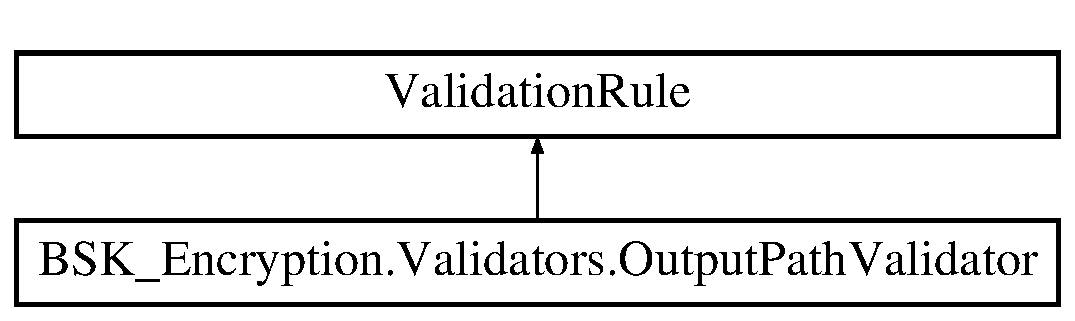
\includegraphics[height=2.000000cm]{class_b_s_k___encryption_1_1_validators_1_1_output_path_validator}
\end{center}
\end{figure}
\subsection*{Public Member Functions}
\begin{DoxyCompactItemize}
\item 
\mbox{\Hypertarget{class_b_s_k___encryption_1_1_validators_1_1_output_path_validator_a68ea16176e6d88f8d419d73973085e03}\label{class_b_s_k___encryption_1_1_validators_1_1_output_path_validator_a68ea16176e6d88f8d419d73973085e03}} 
override Validation\+Result {\bfseries Validate} (object value, Culture\+Info culture\+Info)
\end{DoxyCompactItemize}


\subsection{Detailed Description}
Validation for output path. 



The documentation for this class was generated from the following file\+:\begin{DoxyCompactItemize}
\item 
B\+S\+K\+\_\+\+Encryption/\+Validators/Output\+Path\+Validator.\+cs\end{DoxyCompactItemize}

\hypertarget{class_b_s_k___encryption_1_1_windows_1_1_register_window}{}\section{B\+S\+K\+\_\+\+Encryption.\+Windows.\+Register\+Window Class Reference}
\label{class_b_s_k___encryption_1_1_windows_1_1_register_window}\index{B\+S\+K\+\_\+\+Encryption.\+Windows.\+Register\+Window@{B\+S\+K\+\_\+\+Encryption.\+Windows.\+Register\+Window}}


\mbox{\hyperlink{class_b_s_k___encryption_1_1_windows_1_1_register_window}{Register\+Window}}  


Inheritance diagram for B\+S\+K\+\_\+\+Encryption.\+Windows.\+Register\+Window\+:\begin{figure}[H]
\begin{center}
\leavevmode
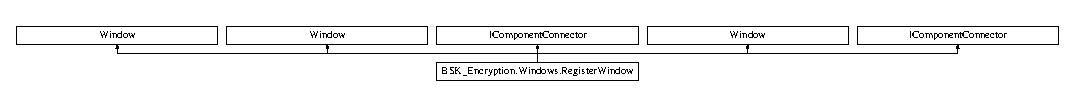
\includegraphics[height=0.861538cm]{class_b_s_k___encryption_1_1_windows_1_1_register_window}
\end{center}
\end{figure}
\subsection*{Public Member Functions}
\begin{DoxyCompactItemize}
\item 
void \mbox{\hyperlink{class_b_s_k___encryption_1_1_windows_1_1_register_window_a69ecfe0446850b9367f2a84191c9236c}{Initialize\+Component}} ()
\begin{DoxyCompactList}\small\item\em Initialize\+Component \end{DoxyCompactList}\item 
void \mbox{\hyperlink{class_b_s_k___encryption_1_1_windows_1_1_register_window_a69ecfe0446850b9367f2a84191c9236c}{Initialize\+Component}} ()
\begin{DoxyCompactList}\small\item\em Initialize\+Component \end{DoxyCompactList}\end{DoxyCompactItemize}


\subsection{Detailed Description}
\mbox{\hyperlink{class_b_s_k___encryption_1_1_windows_1_1_register_window}{Register\+Window}} 

Interaction logic for Register\+Window.\+xaml 

\subsection{Member Function Documentation}
\mbox{\Hypertarget{class_b_s_k___encryption_1_1_windows_1_1_register_window_a69ecfe0446850b9367f2a84191c9236c}\label{class_b_s_k___encryption_1_1_windows_1_1_register_window_a69ecfe0446850b9367f2a84191c9236c}} 
\index{B\+S\+K\+\_\+\+Encryption\+::\+Windows\+::\+Register\+Window@{B\+S\+K\+\_\+\+Encryption\+::\+Windows\+::\+Register\+Window}!Initialize\+Component@{Initialize\+Component}}
\index{Initialize\+Component@{Initialize\+Component}!B\+S\+K\+\_\+\+Encryption\+::\+Windows\+::\+Register\+Window@{B\+S\+K\+\_\+\+Encryption\+::\+Windows\+::\+Register\+Window}}
\subsubsection{\texorpdfstring{Initialize\+Component()}{InitializeComponent()}\hspace{0.1cm}{\footnotesize\ttfamily [1/2]}}
{\footnotesize\ttfamily void B\+S\+K\+\_\+\+Encryption.\+Windows.\+Register\+Window.\+Initialize\+Component (\begin{DoxyParamCaption}{ }\end{DoxyParamCaption})}



Initialize\+Component 

\mbox{\Hypertarget{class_b_s_k___encryption_1_1_windows_1_1_register_window_a69ecfe0446850b9367f2a84191c9236c}\label{class_b_s_k___encryption_1_1_windows_1_1_register_window_a69ecfe0446850b9367f2a84191c9236c}} 
\index{B\+S\+K\+\_\+\+Encryption\+::\+Windows\+::\+Register\+Window@{B\+S\+K\+\_\+\+Encryption\+::\+Windows\+::\+Register\+Window}!Initialize\+Component@{Initialize\+Component}}
\index{Initialize\+Component@{Initialize\+Component}!B\+S\+K\+\_\+\+Encryption\+::\+Windows\+::\+Register\+Window@{B\+S\+K\+\_\+\+Encryption\+::\+Windows\+::\+Register\+Window}}
\subsubsection{\texorpdfstring{Initialize\+Component()}{InitializeComponent()}\hspace{0.1cm}{\footnotesize\ttfamily [2/2]}}
{\footnotesize\ttfamily void B\+S\+K\+\_\+\+Encryption.\+Windows.\+Register\+Window.\+Initialize\+Component (\begin{DoxyParamCaption}{ }\end{DoxyParamCaption})}



Initialize\+Component 



The documentation for this class was generated from the following files\+:\begin{DoxyCompactItemize}
\item 
B\+S\+K\+\_\+\+Encryption/obj/\+Debug/\+Windows/Register\+Window.\+g.\+cs\item 
B\+S\+K\+\_\+\+Encryption/obj/\+Debug/\+Windows/Register\+Window.\+g.\+i.\+cs\item 
B\+S\+K\+\_\+\+Encryption/\+Windows/Register\+Window.\+xaml.\+cs\end{DoxyCompactItemize}

\hypertarget{class_b_s_k___encryption_1_1_encryption_1_1_rsa_encryption_api}{}\section{B\+S\+K\+\_\+\+Encryption.\+Encryption.\+Rsa\+Encryption\+Api Class Reference}
\label{class_b_s_k___encryption_1_1_encryption_1_1_rsa_encryption_api}\index{B\+S\+K\+\_\+\+Encryption.\+Encryption.\+Rsa\+Encryption\+Api@{B\+S\+K\+\_\+\+Encryption.\+Encryption.\+Rsa\+Encryption\+Api}}


Api that handles Rsa \mbox{\hyperlink{namespace_b_s_k___encryption_1_1_encryption}{Encryption}} using keys for given user. \mbox{\hyperlink{namespace_b_s_k___encryption_1_1_encryption}{Encryption}} many to one.  


\subsection*{Static Public Member Functions}
\begin{DoxyCompactItemize}
\item 
static byte \mbox{[}$\,$\mbox{]} \mbox{\hyperlink{class_b_s_k___encryption_1_1_encryption_1_1_rsa_encryption_api_a60bd2ada99112276d7b50b6096269187}{Encrypte}} (byte\mbox{[}$\,$\mbox{]} data, string username)
\begin{DoxyCompactList}\small\item\em Encrypt data using username public key. \end{DoxyCompactList}\item 
static byte \mbox{[}$\,$\mbox{]} \mbox{\hyperlink{class_b_s_k___encryption_1_1_encryption_1_1_rsa_encryption_api_ab085345c3144ba43e1dba49795f7faeb}{Decrypte}} (byte\mbox{[}$\,$\mbox{]} data, string username, byte\mbox{[}$\,$\mbox{]} key\+Pharse)
\begin{DoxyCompactList}\small\item\em Decrypt data using username private key. \end{DoxyCompactList}\item 
static void \mbox{\hyperlink{class_b_s_k___encryption_1_1_encryption_1_1_rsa_encryption_api_a9487324e4e7f5f3e112f4fcd56551102}{Generate\+Key}} (string username, byte\mbox{[}$\,$\mbox{]} key\+Pharse)
\begin{DoxyCompactList}\small\item\em Generate key and save it. \end{DoxyCompactList}\end{DoxyCompactItemize}


\subsection{Detailed Description}
Api that handles Rsa \mbox{\hyperlink{namespace_b_s_k___encryption_1_1_encryption}{Encryption}} using keys for given user. \mbox{\hyperlink{namespace_b_s_k___encryption_1_1_encryption}{Encryption}} many to one. 



\subsection{Member Function Documentation}
\mbox{\Hypertarget{class_b_s_k___encryption_1_1_encryption_1_1_rsa_encryption_api_ab085345c3144ba43e1dba49795f7faeb}\label{class_b_s_k___encryption_1_1_encryption_1_1_rsa_encryption_api_ab085345c3144ba43e1dba49795f7faeb}} 
\index{B\+S\+K\+\_\+\+Encryption\+::\+Encryption\+::\+Rsa\+Encryption\+Api@{B\+S\+K\+\_\+\+Encryption\+::\+Encryption\+::\+Rsa\+Encryption\+Api}!Decrypte@{Decrypte}}
\index{Decrypte@{Decrypte}!B\+S\+K\+\_\+\+Encryption\+::\+Encryption\+::\+Rsa\+Encryption\+Api@{B\+S\+K\+\_\+\+Encryption\+::\+Encryption\+::\+Rsa\+Encryption\+Api}}
\subsubsection{\texorpdfstring{Decrypte()}{Decrypte()}}
{\footnotesize\ttfamily static byte \mbox{[}$\,$\mbox{]} B\+S\+K\+\_\+\+Encryption.\+Encryption.\+Rsa\+Encryption\+Api.\+Decrypte (\begin{DoxyParamCaption}\item[{byte \mbox{[}$\,$\mbox{]}}]{data,  }\item[{string}]{username,  }\item[{byte \mbox{[}$\,$\mbox{]}}]{key\+Pharse }\end{DoxyParamCaption})\hspace{0.3cm}{\ttfamily [static]}}



Decrypt data using username private key. 


\begin{DoxyParams}{Parameters}
{\em data} & Data to decrypt(session key).\\
\hline
{\em username} & Allowed user\\
\hline
{\em key\+Pharse} & Key to decrypt private key\\
\hline
\end{DoxyParams}
\begin{DoxyReturn}{Returns}
Decrypted data.
\end{DoxyReturn}
\mbox{\Hypertarget{class_b_s_k___encryption_1_1_encryption_1_1_rsa_encryption_api_a60bd2ada99112276d7b50b6096269187}\label{class_b_s_k___encryption_1_1_encryption_1_1_rsa_encryption_api_a60bd2ada99112276d7b50b6096269187}} 
\index{B\+S\+K\+\_\+\+Encryption\+::\+Encryption\+::\+Rsa\+Encryption\+Api@{B\+S\+K\+\_\+\+Encryption\+::\+Encryption\+::\+Rsa\+Encryption\+Api}!Encrypte@{Encrypte}}
\index{Encrypte@{Encrypte}!B\+S\+K\+\_\+\+Encryption\+::\+Encryption\+::\+Rsa\+Encryption\+Api@{B\+S\+K\+\_\+\+Encryption\+::\+Encryption\+::\+Rsa\+Encryption\+Api}}
\subsubsection{\texorpdfstring{Encrypte()}{Encrypte()}}
{\footnotesize\ttfamily static byte \mbox{[}$\,$\mbox{]} B\+S\+K\+\_\+\+Encryption.\+Encryption.\+Rsa\+Encryption\+Api.\+Encrypte (\begin{DoxyParamCaption}\item[{byte \mbox{[}$\,$\mbox{]}}]{data,  }\item[{string}]{username }\end{DoxyParamCaption})\hspace{0.3cm}{\ttfamily [static]}}



Encrypt data using username public key. 


\begin{DoxyParams}{Parameters}
{\em data} & Data to encrypt(session key).\\
\hline
{\em username} & Destination user\\
\hline
\end{DoxyParams}
\begin{DoxyReturn}{Returns}
Encrypted data.
\end{DoxyReturn}
\mbox{\Hypertarget{class_b_s_k___encryption_1_1_encryption_1_1_rsa_encryption_api_a9487324e4e7f5f3e112f4fcd56551102}\label{class_b_s_k___encryption_1_1_encryption_1_1_rsa_encryption_api_a9487324e4e7f5f3e112f4fcd56551102}} 
\index{B\+S\+K\+\_\+\+Encryption\+::\+Encryption\+::\+Rsa\+Encryption\+Api@{B\+S\+K\+\_\+\+Encryption\+::\+Encryption\+::\+Rsa\+Encryption\+Api}!Generate\+Key@{Generate\+Key}}
\index{Generate\+Key@{Generate\+Key}!B\+S\+K\+\_\+\+Encryption\+::\+Encryption\+::\+Rsa\+Encryption\+Api@{B\+S\+K\+\_\+\+Encryption\+::\+Encryption\+::\+Rsa\+Encryption\+Api}}
\subsubsection{\texorpdfstring{Generate\+Key()}{GenerateKey()}}
{\footnotesize\ttfamily static void B\+S\+K\+\_\+\+Encryption.\+Encryption.\+Rsa\+Encryption\+Api.\+Generate\+Key (\begin{DoxyParamCaption}\item[{string}]{username,  }\item[{byte \mbox{[}$\,$\mbox{]}}]{key\+Pharse }\end{DoxyParamCaption})\hspace{0.3cm}{\ttfamily [static]}}



Generate key and save it. 


\begin{DoxyParams}{Parameters}
{\em username} & Name of the key owner.\\
\hline
{\em key\+Pharse} & Key to encrypt private key\\
\hline
\end{DoxyParams}


The documentation for this class was generated from the following file\+:\begin{DoxyCompactItemize}
\item 
B\+S\+K\+\_\+\+Encryption/\+Encryption/Rsa\+Encryption\+Api.\+cs\end{DoxyCompactItemize}

\hypertarget{class_b_s_k___encryption_1_1_encryption_1_1_s_h_a256_encryption_api}{}\section{B\+S\+K\+\_\+\+Encryption.\+Encryption.\+S\+H\+A256\+Encryption\+Api Class Reference}
\label{class_b_s_k___encryption_1_1_encryption_1_1_s_h_a256_encryption_api}\index{B\+S\+K\+\_\+\+Encryption.\+Encryption.\+S\+H\+A256\+Encryption\+Api@{B\+S\+K\+\_\+\+Encryption.\+Encryption.\+S\+H\+A256\+Encryption\+Api}}


Api that handles the hasing method.  


\subsection*{Static Public Member Functions}
\begin{DoxyCompactItemize}
\item 
static byte \mbox{[}$\,$\mbox{]} \mbox{\hyperlink{class_b_s_k___encryption_1_1_encryption_1_1_s_h_a256_encryption_api_a3892e8fa36b63070cae039ac8d2981eb}{get\+Hash\+Sha256}} (string key\+Pharse)
\begin{DoxyCompactList}\small\item\em Hash the data using S\+H\+A-\/256. \end{DoxyCompactList}\end{DoxyCompactItemize}


\subsection{Detailed Description}
Api that handles the hasing method. 



\subsection{Member Function Documentation}
\mbox{\Hypertarget{class_b_s_k___encryption_1_1_encryption_1_1_s_h_a256_encryption_api_a3892e8fa36b63070cae039ac8d2981eb}\label{class_b_s_k___encryption_1_1_encryption_1_1_s_h_a256_encryption_api_a3892e8fa36b63070cae039ac8d2981eb}} 
\index{B\+S\+K\+\_\+\+Encryption\+::\+Encryption\+::\+S\+H\+A256\+Encryption\+Api@{B\+S\+K\+\_\+\+Encryption\+::\+Encryption\+::\+S\+H\+A256\+Encryption\+Api}!get\+Hash\+Sha256@{get\+Hash\+Sha256}}
\index{get\+Hash\+Sha256@{get\+Hash\+Sha256}!B\+S\+K\+\_\+\+Encryption\+::\+Encryption\+::\+S\+H\+A256\+Encryption\+Api@{B\+S\+K\+\_\+\+Encryption\+::\+Encryption\+::\+S\+H\+A256\+Encryption\+Api}}
\subsubsection{\texorpdfstring{get\+Hash\+Sha256()}{getHashSha256()}}
{\footnotesize\ttfamily static byte \mbox{[}$\,$\mbox{]} B\+S\+K\+\_\+\+Encryption.\+Encryption.\+S\+H\+A256\+Encryption\+Api.\+get\+Hash\+Sha256 (\begin{DoxyParamCaption}\item[{string}]{key\+Pharse }\end{DoxyParamCaption})\hspace{0.3cm}{\ttfamily [static]}}



Hash the data using S\+H\+A-\/256. 


\begin{DoxyParams}{Parameters}
{\em key\+Pharse} & String to be hashed(keypharse for private key).\\
\hline
\end{DoxyParams}
\begin{DoxyReturn}{Returns}
Hashed data.
\end{DoxyReturn}


The documentation for this class was generated from the following file\+:\begin{DoxyCompactItemize}
\item 
B\+S\+K\+\_\+\+Encryption/\+Encryption/S\+H\+A256\+Encryption\+Api.\+cs\end{DoxyCompactItemize}

\hypertarget{class_b_s_k___encryption_1_1_validators_1_1_text_validator}{}\section{B\+S\+K\+\_\+\+Encryption.\+Validators.\+Text\+Validator Class Reference}
\label{class_b_s_k___encryption_1_1_validators_1_1_text_validator}\index{B\+S\+K\+\_\+\+Encryption.\+Validators.\+Text\+Validator@{B\+S\+K\+\_\+\+Encryption.\+Validators.\+Text\+Validator}}


Validation for path if aren\textquotesingle{}t empty or null.  


Inheritance diagram for B\+S\+K\+\_\+\+Encryption.\+Validators.\+Text\+Validator\+:\begin{figure}[H]
\begin{center}
\leavevmode
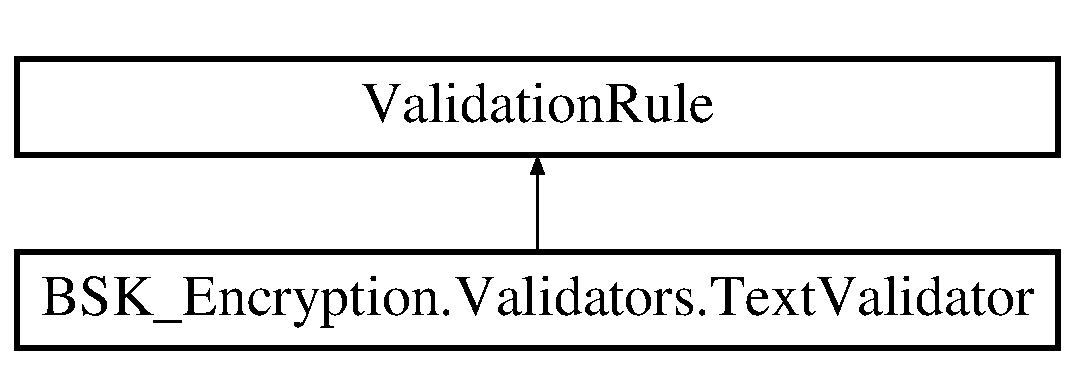
\includegraphics[height=2.000000cm]{class_b_s_k___encryption_1_1_validators_1_1_text_validator}
\end{center}
\end{figure}
\subsection*{Public Member Functions}
\begin{DoxyCompactItemize}
\item 
\mbox{\Hypertarget{class_b_s_k___encryption_1_1_validators_1_1_text_validator_a315e01771c92cefc430ca65a53f8b148}\label{class_b_s_k___encryption_1_1_validators_1_1_text_validator_a315e01771c92cefc430ca65a53f8b148}} 
override Validation\+Result {\bfseries Validate} (object value, Culture\+Info culture\+Info)
\end{DoxyCompactItemize}


\subsection{Detailed Description}
Validation for path if aren\textquotesingle{}t empty or null. 



The documentation for this class was generated from the following file\+:\begin{DoxyCompactItemize}
\item 
B\+S\+K\+\_\+\+Encryption/\+Validators/Text\+Validator.\+cs\end{DoxyCompactItemize}

\hypertarget{class_b_s_k___encryption_1_1_encryption_1_1_user}{}\section{B\+S\+K\+\_\+\+Encryption.\+Encryption.\+User Class Reference}
\label{class_b_s_k___encryption_1_1_encryption_1_1_user}\index{B\+S\+K\+\_\+\+Encryption.\+Encryption.\+User@{B\+S\+K\+\_\+\+Encryption.\+Encryption.\+User}}


Container for user/\+Rsa\+\_\+password manage.  


\subsection*{Public Member Functions}
\begin{DoxyCompactItemize}
\item 
\mbox{\Hypertarget{class_b_s_k___encryption_1_1_encryption_1_1_user_aa527816e42c0943ef512e6556faf3563}\label{class_b_s_k___encryption_1_1_encryption_1_1_user_aa527816e42c0943ef512e6556faf3563}} 
{\bfseries User} (string name)
\item 
void \mbox{\hyperlink{class_b_s_k___encryption_1_1_encryption_1_1_user_a881a5e8ff2f140aa2c05be2213522a5f}{Write\+To\+Xml}} (Xml\+Writer output)
\begin{DoxyCompactList}\small\item\em Writes user from xml file. \end{DoxyCompactList}\item 
void \mbox{\hyperlink{class_b_s_k___encryption_1_1_encryption_1_1_user_a7f44735ece5103022d100d3b5780e82d}{Store\+Key}} (byte\mbox{[}$\,$\mbox{]} key)
\begin{DoxyCompactList}\small\item\em Encrypt with public key and store the session key. \end{DoxyCompactList}\item 
byte \mbox{[}$\,$\mbox{]} \mbox{\hyperlink{class_b_s_k___encryption_1_1_encryption_1_1_user_a60bacb1a794eae94f4f38e3fc3801e03}{Load\+Key}} (string key\+Pharse)
\begin{DoxyCompactList}\small\item\em Decrypt with private key. \end{DoxyCompactList}\end{DoxyCompactItemize}
\subsection*{Static Public Member Functions}
\begin{DoxyCompactItemize}
\item 
static \mbox{\hyperlink{class_b_s_k___encryption_1_1_encryption_1_1_user}{User}} \mbox{\hyperlink{class_b_s_k___encryption_1_1_encryption_1_1_user_ae5f1c5220e3588843a0cd2850d8bf61a}{From\+Xml}} (Xml\+Reader input)
\begin{DoxyCompactList}\small\item\em Load config for user from xml file. \end{DoxyCompactList}\end{DoxyCompactItemize}
\subsection*{Properties}
\begin{DoxyCompactItemize}
\item 
string \mbox{\hyperlink{class_b_s_k___encryption_1_1_encryption_1_1_user_a00edfd3ff33285f11bc3dfdb2657f2a9}{Name}}\hspace{0.3cm}{\ttfamily  \mbox{[}get\mbox{]}}
\begin{DoxyCompactList}\small\item\em Name of the user. \end{DoxyCompactList}\end{DoxyCompactItemize}


\subsection{Detailed Description}
Container for user/\+Rsa\+\_\+password manage. 



\subsection{Member Function Documentation}
\mbox{\Hypertarget{class_b_s_k___encryption_1_1_encryption_1_1_user_ae5f1c5220e3588843a0cd2850d8bf61a}\label{class_b_s_k___encryption_1_1_encryption_1_1_user_ae5f1c5220e3588843a0cd2850d8bf61a}} 
\index{B\+S\+K\+\_\+\+Encryption\+::\+Encryption\+::\+User@{B\+S\+K\+\_\+\+Encryption\+::\+Encryption\+::\+User}!From\+Xml@{From\+Xml}}
\index{From\+Xml@{From\+Xml}!B\+S\+K\+\_\+\+Encryption\+::\+Encryption\+::\+User@{B\+S\+K\+\_\+\+Encryption\+::\+Encryption\+::\+User}}
\subsubsection{\texorpdfstring{From\+Xml()}{FromXml()}}
{\footnotesize\ttfamily static \mbox{\hyperlink{class_b_s_k___encryption_1_1_encryption_1_1_user}{User}} B\+S\+K\+\_\+\+Encryption.\+Encryption.\+User.\+From\+Xml (\begin{DoxyParamCaption}\item[{Xml\+Reader}]{input }\end{DoxyParamCaption})\hspace{0.3cm}{\ttfamily [static]}}



Load config for user from xml file. 


\begin{DoxyParams}{Parameters}
{\em input} & Opened xml file.\\
\hline
\end{DoxyParams}
\begin{DoxyReturn}{Returns}
Object of type {\ttfamily \mbox{\hyperlink{class_b_s_k___encryption_1_1_encryption_1_1_user}{User}}} deserilized from file.
\end{DoxyReturn}
\mbox{\Hypertarget{class_b_s_k___encryption_1_1_encryption_1_1_user_a60bacb1a794eae94f4f38e3fc3801e03}\label{class_b_s_k___encryption_1_1_encryption_1_1_user_a60bacb1a794eae94f4f38e3fc3801e03}} 
\index{B\+S\+K\+\_\+\+Encryption\+::\+Encryption\+::\+User@{B\+S\+K\+\_\+\+Encryption\+::\+Encryption\+::\+User}!Load\+Key@{Load\+Key}}
\index{Load\+Key@{Load\+Key}!B\+S\+K\+\_\+\+Encryption\+::\+Encryption\+::\+User@{B\+S\+K\+\_\+\+Encryption\+::\+Encryption\+::\+User}}
\subsubsection{\texorpdfstring{Load\+Key()}{LoadKey()}}
{\footnotesize\ttfamily byte \mbox{[}$\,$\mbox{]} B\+S\+K\+\_\+\+Encryption.\+Encryption.\+User.\+Load\+Key (\begin{DoxyParamCaption}\item[{string}]{key\+Pharse }\end{DoxyParamCaption})}



Decrypt with private key. 


\begin{DoxyParams}{Parameters}
{\em key\+Pharse} & keypharse to decrypte private key\\
\hline
\end{DoxyParams}
\begin{DoxyReturn}{Returns}
Decrypted session key
\end{DoxyReturn}
\mbox{\Hypertarget{class_b_s_k___encryption_1_1_encryption_1_1_user_a7f44735ece5103022d100d3b5780e82d}\label{class_b_s_k___encryption_1_1_encryption_1_1_user_a7f44735ece5103022d100d3b5780e82d}} 
\index{B\+S\+K\+\_\+\+Encryption\+::\+Encryption\+::\+User@{B\+S\+K\+\_\+\+Encryption\+::\+Encryption\+::\+User}!Store\+Key@{Store\+Key}}
\index{Store\+Key@{Store\+Key}!B\+S\+K\+\_\+\+Encryption\+::\+Encryption\+::\+User@{B\+S\+K\+\_\+\+Encryption\+::\+Encryption\+::\+User}}
\subsubsection{\texorpdfstring{Store\+Key()}{StoreKey()}}
{\footnotesize\ttfamily void B\+S\+K\+\_\+\+Encryption.\+Encryption.\+User.\+Store\+Key (\begin{DoxyParamCaption}\item[{byte \mbox{[}$\,$\mbox{]}}]{key }\end{DoxyParamCaption})}



Encrypt with public key and store the session key. 


\begin{DoxyParams}{Parameters}
{\em key} & Key to be stored in user container.\\
\hline
\end{DoxyParams}
\mbox{\Hypertarget{class_b_s_k___encryption_1_1_encryption_1_1_user_a881a5e8ff2f140aa2c05be2213522a5f}\label{class_b_s_k___encryption_1_1_encryption_1_1_user_a881a5e8ff2f140aa2c05be2213522a5f}} 
\index{B\+S\+K\+\_\+\+Encryption\+::\+Encryption\+::\+User@{B\+S\+K\+\_\+\+Encryption\+::\+Encryption\+::\+User}!Write\+To\+Xml@{Write\+To\+Xml}}
\index{Write\+To\+Xml@{Write\+To\+Xml}!B\+S\+K\+\_\+\+Encryption\+::\+Encryption\+::\+User@{B\+S\+K\+\_\+\+Encryption\+::\+Encryption\+::\+User}}
\subsubsection{\texorpdfstring{Write\+To\+Xml()}{WriteToXml()}}
{\footnotesize\ttfamily void B\+S\+K\+\_\+\+Encryption.\+Encryption.\+User.\+Write\+To\+Xml (\begin{DoxyParamCaption}\item[{Xml\+Writer}]{output }\end{DoxyParamCaption})}



Writes user from xml file. 


\begin{DoxyParams}{Parameters}
{\em output} & Opened xml file.\\
\hline
\end{DoxyParams}


\subsection{Property Documentation}
\mbox{\Hypertarget{class_b_s_k___encryption_1_1_encryption_1_1_user_a00edfd3ff33285f11bc3dfdb2657f2a9}\label{class_b_s_k___encryption_1_1_encryption_1_1_user_a00edfd3ff33285f11bc3dfdb2657f2a9}} 
\index{B\+S\+K\+\_\+\+Encryption\+::\+Encryption\+::\+User@{B\+S\+K\+\_\+\+Encryption\+::\+Encryption\+::\+User}!Name@{Name}}
\index{Name@{Name}!B\+S\+K\+\_\+\+Encryption\+::\+Encryption\+::\+User@{B\+S\+K\+\_\+\+Encryption\+::\+Encryption\+::\+User}}
\subsubsection{\texorpdfstring{Name}{Name}}
{\footnotesize\ttfamily string B\+S\+K\+\_\+\+Encryption.\+Encryption.\+User.\+Name\hspace{0.3cm}{\ttfamily [get]}}



Name of the user. 



The documentation for this class was generated from the following file\+:\begin{DoxyCompactItemize}
\item 
B\+S\+K\+\_\+\+Encryption/\+Encryption/User.\+cs\end{DoxyCompactItemize}

\hypertarget{class_b_s_k___encryption_1_1_view_models_1_1_user_grid_element}{}\section{B\+S\+K\+\_\+\+Encryption.\+View\+Models.\+User\+Grid\+Element Class Reference}
\label{class_b_s_k___encryption_1_1_view_models_1_1_user_grid_element}\index{B\+S\+K\+\_\+\+Encryption.\+View\+Models.\+User\+Grid\+Element@{B\+S\+K\+\_\+\+Encryption.\+View\+Models.\+User\+Grid\+Element}}


Part of Users selection table.  


\subsection*{Public Member Functions}
\begin{DoxyCompactItemize}
\item 
\mbox{\Hypertarget{class_b_s_k___encryption_1_1_view_models_1_1_user_grid_element_a785c9d979f002992926399ff1324b56e}\label{class_b_s_k___encryption_1_1_view_models_1_1_user_grid_element_a785c9d979f002992926399ff1324b56e}} 
{\bfseries User\+Grid\+Element} (string username)
\item 
override bool \mbox{\hyperlink{class_b_s_k___encryption_1_1_view_models_1_1_user_grid_element_a5819f5e5be4cb5d76ceca220683689ce}{Equals}} (object obj)
\begin{DoxyCompactList}\small\item\em Equals by type then by username. \end{DoxyCompactList}\end{DoxyCompactItemize}
\subsection*{Properties}
\begin{DoxyCompactItemize}
\item 
string \mbox{\hyperlink{class_b_s_k___encryption_1_1_view_models_1_1_user_grid_element_a51f91f62aeffe54cd095deb969370f56}{User\+Name}}\hspace{0.3cm}{\ttfamily  \mbox{[}get, set\mbox{]}}
\begin{DoxyCompactList}\small\item\em Login of the user. \end{DoxyCompactList}\item 
bool \mbox{\hyperlink{class_b_s_k___encryption_1_1_view_models_1_1_user_grid_element_ae2897007d40f48fe6267173a84aeac24}{Is\+Checked}}\hspace{0.3cm}{\ttfamily  \mbox{[}get, set\mbox{]}}
\begin{DoxyCompactList}\small\item\em Indicates if will be authorized or not. \end{DoxyCompactList}\end{DoxyCompactItemize}


\subsection{Detailed Description}
Part of Users selection table. 



\subsection{Member Function Documentation}
\mbox{\Hypertarget{class_b_s_k___encryption_1_1_view_models_1_1_user_grid_element_a5819f5e5be4cb5d76ceca220683689ce}\label{class_b_s_k___encryption_1_1_view_models_1_1_user_grid_element_a5819f5e5be4cb5d76ceca220683689ce}} 
\index{B\+S\+K\+\_\+\+Encryption\+::\+View\+Models\+::\+User\+Grid\+Element@{B\+S\+K\+\_\+\+Encryption\+::\+View\+Models\+::\+User\+Grid\+Element}!Equals@{Equals}}
\index{Equals@{Equals}!B\+S\+K\+\_\+\+Encryption\+::\+View\+Models\+::\+User\+Grid\+Element@{B\+S\+K\+\_\+\+Encryption\+::\+View\+Models\+::\+User\+Grid\+Element}}
\subsubsection{\texorpdfstring{Equals()}{Equals()}}
{\footnotesize\ttfamily override bool B\+S\+K\+\_\+\+Encryption.\+View\+Models.\+User\+Grid\+Element.\+Equals (\begin{DoxyParamCaption}\item[{object}]{obj }\end{DoxyParamCaption})}



Equals by type then by username. 


\begin{DoxyParams}{Parameters}
{\em obj} & \\
\hline
\end{DoxyParams}
\begin{DoxyReturn}{Returns}

\end{DoxyReturn}


\subsection{Property Documentation}
\mbox{\Hypertarget{class_b_s_k___encryption_1_1_view_models_1_1_user_grid_element_ae2897007d40f48fe6267173a84aeac24}\label{class_b_s_k___encryption_1_1_view_models_1_1_user_grid_element_ae2897007d40f48fe6267173a84aeac24}} 
\index{B\+S\+K\+\_\+\+Encryption\+::\+View\+Models\+::\+User\+Grid\+Element@{B\+S\+K\+\_\+\+Encryption\+::\+View\+Models\+::\+User\+Grid\+Element}!Is\+Checked@{Is\+Checked}}
\index{Is\+Checked@{Is\+Checked}!B\+S\+K\+\_\+\+Encryption\+::\+View\+Models\+::\+User\+Grid\+Element@{B\+S\+K\+\_\+\+Encryption\+::\+View\+Models\+::\+User\+Grid\+Element}}
\subsubsection{\texorpdfstring{Is\+Checked}{IsChecked}}
{\footnotesize\ttfamily bool B\+S\+K\+\_\+\+Encryption.\+View\+Models.\+User\+Grid\+Element.\+Is\+Checked\hspace{0.3cm}{\ttfamily [get]}, {\ttfamily [set]}}



Indicates if will be authorized or not. 

\mbox{\Hypertarget{class_b_s_k___encryption_1_1_view_models_1_1_user_grid_element_a51f91f62aeffe54cd095deb969370f56}\label{class_b_s_k___encryption_1_1_view_models_1_1_user_grid_element_a51f91f62aeffe54cd095deb969370f56}} 
\index{B\+S\+K\+\_\+\+Encryption\+::\+View\+Models\+::\+User\+Grid\+Element@{B\+S\+K\+\_\+\+Encryption\+::\+View\+Models\+::\+User\+Grid\+Element}!User\+Name@{User\+Name}}
\index{User\+Name@{User\+Name}!B\+S\+K\+\_\+\+Encryption\+::\+View\+Models\+::\+User\+Grid\+Element@{B\+S\+K\+\_\+\+Encryption\+::\+View\+Models\+::\+User\+Grid\+Element}}
\subsubsection{\texorpdfstring{User\+Name}{UserName}}
{\footnotesize\ttfamily string B\+S\+K\+\_\+\+Encryption.\+View\+Models.\+User\+Grid\+Element.\+User\+Name\hspace{0.3cm}{\ttfamily [get]}, {\ttfamily [set]}}



Login of the user. 



The documentation for this class was generated from the following file\+:\begin{DoxyCompactItemize}
\item 
B\+S\+K\+\_\+\+Encryption/\+View\+Models/User\+Grid\+Element.\+cs\end{DoxyCompactItemize}

\hypertarget{class_b_s_k___encryption_1_1_windows_1_1_users_window}{}\section{B\+S\+K\+\_\+\+Encryption.\+Windows.\+Users\+Window Class Reference}
\label{class_b_s_k___encryption_1_1_windows_1_1_users_window}\index{B\+S\+K\+\_\+\+Encryption.\+Windows.\+Users\+Window@{B\+S\+K\+\_\+\+Encryption.\+Windows.\+Users\+Window}}


\mbox{\hyperlink{class_b_s_k___encryption_1_1_windows_1_1_users_window}{Users\+Window}}  


Inheritance diagram for B\+S\+K\+\_\+\+Encryption.\+Windows.\+Users\+Window\+:\begin{figure}[H]
\begin{center}
\leavevmode
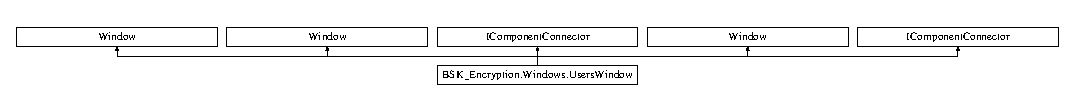
\includegraphics[height=0.910569cm]{class_b_s_k___encryption_1_1_windows_1_1_users_window}
\end{center}
\end{figure}
\subsection*{Public Member Functions}
\begin{DoxyCompactItemize}
\item 
void \mbox{\hyperlink{class_b_s_k___encryption_1_1_windows_1_1_users_window_a2c471ea1e3ac60997266866d55f7b202}{Initialize\+Component}} ()
\begin{DoxyCompactList}\small\item\em Initialize\+Component \end{DoxyCompactList}\item 
void \mbox{\hyperlink{class_b_s_k___encryption_1_1_windows_1_1_users_window_a2c471ea1e3ac60997266866d55f7b202}{Initialize\+Component}} ()
\begin{DoxyCompactList}\small\item\em Initialize\+Component \end{DoxyCompactList}\end{DoxyCompactItemize}


\subsection{Detailed Description}
\mbox{\hyperlink{class_b_s_k___encryption_1_1_windows_1_1_users_window}{Users\+Window}} 

Interaction logic for Users\+Window.\+xaml 

\subsection{Member Function Documentation}
\mbox{\Hypertarget{class_b_s_k___encryption_1_1_windows_1_1_users_window_a2c471ea1e3ac60997266866d55f7b202}\label{class_b_s_k___encryption_1_1_windows_1_1_users_window_a2c471ea1e3ac60997266866d55f7b202}} 
\index{B\+S\+K\+\_\+\+Encryption\+::\+Windows\+::\+Users\+Window@{B\+S\+K\+\_\+\+Encryption\+::\+Windows\+::\+Users\+Window}!Initialize\+Component@{Initialize\+Component}}
\index{Initialize\+Component@{Initialize\+Component}!B\+S\+K\+\_\+\+Encryption\+::\+Windows\+::\+Users\+Window@{B\+S\+K\+\_\+\+Encryption\+::\+Windows\+::\+Users\+Window}}
\subsubsection{\texorpdfstring{Initialize\+Component()}{InitializeComponent()}\hspace{0.1cm}{\footnotesize\ttfamily [1/2]}}
{\footnotesize\ttfamily void B\+S\+K\+\_\+\+Encryption.\+Windows.\+Users\+Window.\+Initialize\+Component (\begin{DoxyParamCaption}{ }\end{DoxyParamCaption})}



Initialize\+Component 

\mbox{\Hypertarget{class_b_s_k___encryption_1_1_windows_1_1_users_window_a2c471ea1e3ac60997266866d55f7b202}\label{class_b_s_k___encryption_1_1_windows_1_1_users_window_a2c471ea1e3ac60997266866d55f7b202}} 
\index{B\+S\+K\+\_\+\+Encryption\+::\+Windows\+::\+Users\+Window@{B\+S\+K\+\_\+\+Encryption\+::\+Windows\+::\+Users\+Window}!Initialize\+Component@{Initialize\+Component}}
\index{Initialize\+Component@{Initialize\+Component}!B\+S\+K\+\_\+\+Encryption\+::\+Windows\+::\+Users\+Window@{B\+S\+K\+\_\+\+Encryption\+::\+Windows\+::\+Users\+Window}}
\subsubsection{\texorpdfstring{Initialize\+Component()}{InitializeComponent()}\hspace{0.1cm}{\footnotesize\ttfamily [2/2]}}
{\footnotesize\ttfamily void B\+S\+K\+\_\+\+Encryption.\+Windows.\+Users\+Window.\+Initialize\+Component (\begin{DoxyParamCaption}{ }\end{DoxyParamCaption})}



Initialize\+Component 



The documentation for this class was generated from the following files\+:\begin{DoxyCompactItemize}
\item 
B\+S\+K\+\_\+\+Encryption/obj/\+Debug/\+Windows/Users\+Window.\+g.\+cs\item 
B\+S\+K\+\_\+\+Encryption/obj/\+Debug/\+Windows/Users\+Window.\+g.\+i.\+cs\item 
B\+S\+K\+\_\+\+Encryption/\+Windows/Users\+Window.\+xaml.\+cs\end{DoxyCompactItemize}

\hypertarget{class_b_s_k___encryption_1_1_view_models_1_1_user_view_model}{}\section{B\+S\+K\+\_\+\+Encryption.\+View\+Models.\+User\+View\+Model Class Reference}
\label{class_b_s_k___encryption_1_1_view_models_1_1_user_view_model}\index{B\+S\+K\+\_\+\+Encryption.\+View\+Models.\+User\+View\+Model@{B\+S\+K\+\_\+\+Encryption.\+View\+Models.\+User\+View\+Model}}


Singleton to remember authorized users in process.  


\subsection*{Properties}
\begin{DoxyCompactItemize}
\item 
\mbox{\Hypertarget{class_b_s_k___encryption_1_1_view_models_1_1_user_view_model_aa1f873290abb17312273776823dd5723}\label{class_b_s_k___encryption_1_1_view_models_1_1_user_view_model_aa1f873290abb17312273776823dd5723}} 
static \mbox{\hyperlink{class_b_s_k___encryption_1_1_view_models_1_1_user_view_model}{User\+View\+Model}} {\bfseries Instance}\hspace{0.3cm}{\ttfamily  \mbox{[}get\mbox{]}}
\item 
\mbox{\Hypertarget{class_b_s_k___encryption_1_1_view_models_1_1_user_view_model_ac7ac65701eccd6a6f03e2f59817bf8ca}\label{class_b_s_k___encryption_1_1_view_models_1_1_user_view_model_ac7ac65701eccd6a6f03e2f59817bf8ca}} 
Observable\+Collection$<$ \mbox{\hyperlink{class_b_s_k___encryption_1_1_view_models_1_1_user_grid_element}{User\+Grid\+Element}} $>$ {\bfseries All\+Users}\hspace{0.3cm}{\ttfamily  \mbox{[}get, set\mbox{]}}
\end{DoxyCompactItemize}


\subsection{Detailed Description}
Singleton to remember authorized users in process. 



The documentation for this class was generated from the following file\+:\begin{DoxyCompactItemize}
\item 
B\+S\+K\+\_\+\+Encryption/\+View\+Models/User\+View\+Model.\+cs\end{DoxyCompactItemize}

\hypertarget{class_b_s_k___encryption_1_1_encryption_1_1_o_f_b_1_1_zero_stream}{}\section{B\+S\+K\+\_\+\+Encryption.\+Encryption.\+O\+F\+B.\+Zero\+Stream Class Reference}
\label{class_b_s_k___encryption_1_1_encryption_1_1_o_f_b_1_1_zero_stream}\index{B\+S\+K\+\_\+\+Encryption.\+Encryption.\+O\+F\+B.\+Zero\+Stream@{B\+S\+K\+\_\+\+Encryption.\+Encryption.\+O\+F\+B.\+Zero\+Stream}}


Infinite Stream tha gives always zeros.  


Inheritance diagram for B\+S\+K\+\_\+\+Encryption.\+Encryption.\+O\+F\+B.\+Zero\+Stream\+:\begin{figure}[H]
\begin{center}
\leavevmode
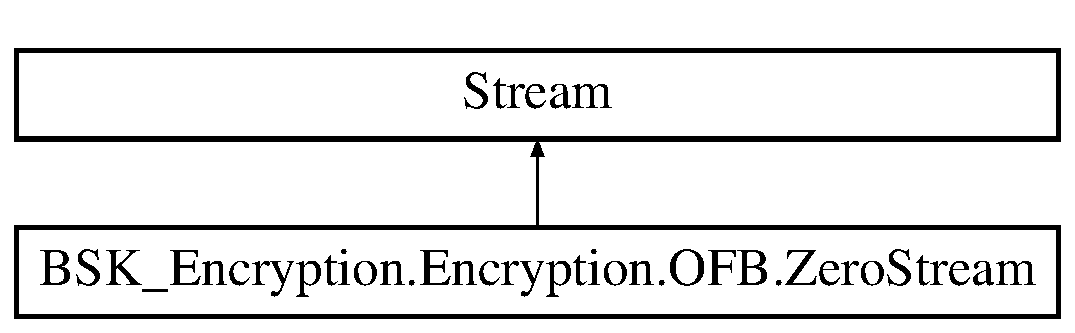
\includegraphics[height=2.000000cm]{class_b_s_k___encryption_1_1_encryption_1_1_o_f_b_1_1_zero_stream}
\end{center}
\end{figure}
\subsection*{Public Member Functions}
\begin{DoxyCompactItemize}
\item 
\mbox{\Hypertarget{class_b_s_k___encryption_1_1_encryption_1_1_o_f_b_1_1_zero_stream_a48a7f982b8a029dd87eba9bd79822d16}\label{class_b_s_k___encryption_1_1_encryption_1_1_o_f_b_1_1_zero_stream_a48a7f982b8a029dd87eba9bd79822d16}} 
override int {\bfseries Read} (byte\mbox{[}$\,$\mbox{]} buffer, int offset, int count)
\item 
\mbox{\Hypertarget{class_b_s_k___encryption_1_1_encryption_1_1_o_f_b_1_1_zero_stream_a6c79205edc2aea33e6d6b314e6e002c8}\label{class_b_s_k___encryption_1_1_encryption_1_1_o_f_b_1_1_zero_stream_a6c79205edc2aea33e6d6b314e6e002c8}} 
override void {\bfseries Flush} ()
\item 
\mbox{\Hypertarget{class_b_s_k___encryption_1_1_encryption_1_1_o_f_b_1_1_zero_stream_a2523d01afb53df768fd3e09e3b565fec}\label{class_b_s_k___encryption_1_1_encryption_1_1_o_f_b_1_1_zero_stream_a2523d01afb53df768fd3e09e3b565fec}} 
override long {\bfseries Seek} (long offset, Seek\+Origin origin)
\item 
\mbox{\Hypertarget{class_b_s_k___encryption_1_1_encryption_1_1_o_f_b_1_1_zero_stream_aa98fad7a1c99b11dd7a12bf73ea51203}\label{class_b_s_k___encryption_1_1_encryption_1_1_o_f_b_1_1_zero_stream_aa98fad7a1c99b11dd7a12bf73ea51203}} 
override void {\bfseries Set\+Length} (long value)
\item 
\mbox{\Hypertarget{class_b_s_k___encryption_1_1_encryption_1_1_o_f_b_1_1_zero_stream_a18edb32e349ca66981c9ab7cfc6c1c5d}\label{class_b_s_k___encryption_1_1_encryption_1_1_o_f_b_1_1_zero_stream_a18edb32e349ca66981c9ab7cfc6c1c5d}} 
override void {\bfseries Write} (byte\mbox{[}$\,$\mbox{]} buffer, int offset, int count)
\end{DoxyCompactItemize}
\subsection*{Properties}
\begin{DoxyCompactItemize}
\item 
\mbox{\Hypertarget{class_b_s_k___encryption_1_1_encryption_1_1_o_f_b_1_1_zero_stream_af2f1571c15481ab5ae68ef15e146f2a0}\label{class_b_s_k___encryption_1_1_encryption_1_1_o_f_b_1_1_zero_stream_af2f1571c15481ab5ae68ef15e146f2a0}} 
override bool {\bfseries Can\+Read}\hspace{0.3cm}{\ttfamily  \mbox{[}get\mbox{]}}
\item 
\mbox{\Hypertarget{class_b_s_k___encryption_1_1_encryption_1_1_o_f_b_1_1_zero_stream_a5692e8759711504610ab938c72550860}\label{class_b_s_k___encryption_1_1_encryption_1_1_o_f_b_1_1_zero_stream_a5692e8759711504610ab938c72550860}} 
override bool {\bfseries Can\+Seek}\hspace{0.3cm}{\ttfamily  \mbox{[}get\mbox{]}}
\item 
\mbox{\Hypertarget{class_b_s_k___encryption_1_1_encryption_1_1_o_f_b_1_1_zero_stream_ad8eb981bca8f777a03027a482500eaef}\label{class_b_s_k___encryption_1_1_encryption_1_1_o_f_b_1_1_zero_stream_ad8eb981bca8f777a03027a482500eaef}} 
override bool {\bfseries Can\+Write}\hspace{0.3cm}{\ttfamily  \mbox{[}get\mbox{]}}
\item 
\mbox{\Hypertarget{class_b_s_k___encryption_1_1_encryption_1_1_o_f_b_1_1_zero_stream_a5923a6c8a9767862fc83546950bc467e}\label{class_b_s_k___encryption_1_1_encryption_1_1_o_f_b_1_1_zero_stream_a5923a6c8a9767862fc83546950bc467e}} 
override long {\bfseries Length}\hspace{0.3cm}{\ttfamily  \mbox{[}get\mbox{]}}
\item 
\mbox{\Hypertarget{class_b_s_k___encryption_1_1_encryption_1_1_o_f_b_1_1_zero_stream_a4a54dd7cb54404fd11ab65986e8b3dd9}\label{class_b_s_k___encryption_1_1_encryption_1_1_o_f_b_1_1_zero_stream_a4a54dd7cb54404fd11ab65986e8b3dd9}} 
override long {\bfseries Position}\hspace{0.3cm}{\ttfamily  \mbox{[}get, set\mbox{]}}
\end{DoxyCompactItemize}


\subsection{Detailed Description}
Infinite Stream tha gives always zeros. 



The documentation for this class was generated from the following file\+:\begin{DoxyCompactItemize}
\item 
B\+S\+K\+\_\+\+Encryption/\+Encryption/\+O\+F\+B/Zero\+Stream.\+cs\end{DoxyCompactItemize}

%--- End generated contents ---

% Index
\backmatter
\newpage
\phantomsection
\clearemptydoublepage
\addcontentsline{toc}{chapter}{Index}
\printindex

\end{document}
